This appendix provides  truth level distributions for $b$-jets and extra jets in 
the \ttbar\ and $Wt$ events.  Predictions obtained with {\sc Powheg+Pythia} hdamp=$\infty$, 
{\sc MC@NLO+Herwig}, {\sc Powheg+Pythia} hdamp=$m_{top}$ and  {\sc MadGraph+Pythia} are presented.
\subsection{Jet distributions for $\ttbar$ events}
Figure~\ref{fig:truthbjet} shows the \pt\ and $\eta$ distributions for $b$-jets and for extra jets obtained
using different \ttbar\  event generators.  
The $b$-jet \pt\ and $\eta$ distributions obtained with different generators agree to within a few per cent.  
MC@NLO has a broader $\eta$ distributon for extra jets than the other generators.
Figure~\ref{fig:ntruthjets} presents the extra jet multiplicity
distributions for the generators, with several choices for the minimum jet \pt.
Differences among the generators as large as 40\%\  are seen for
extra jet multiplicities $\ge 5$.  
The extra jet \pt\ spectra for jets of rank 1 through rank 5 are shown in Figure~\ref{fig:truthjetpt}.
Differences up to 20\%\ for the leading jet and up to 40\%\ for higher rank jets are seen at high jet transverse
momentum.

\begin{figure}
\centering
\begin{subfigure}[]{0.45\textwidth}
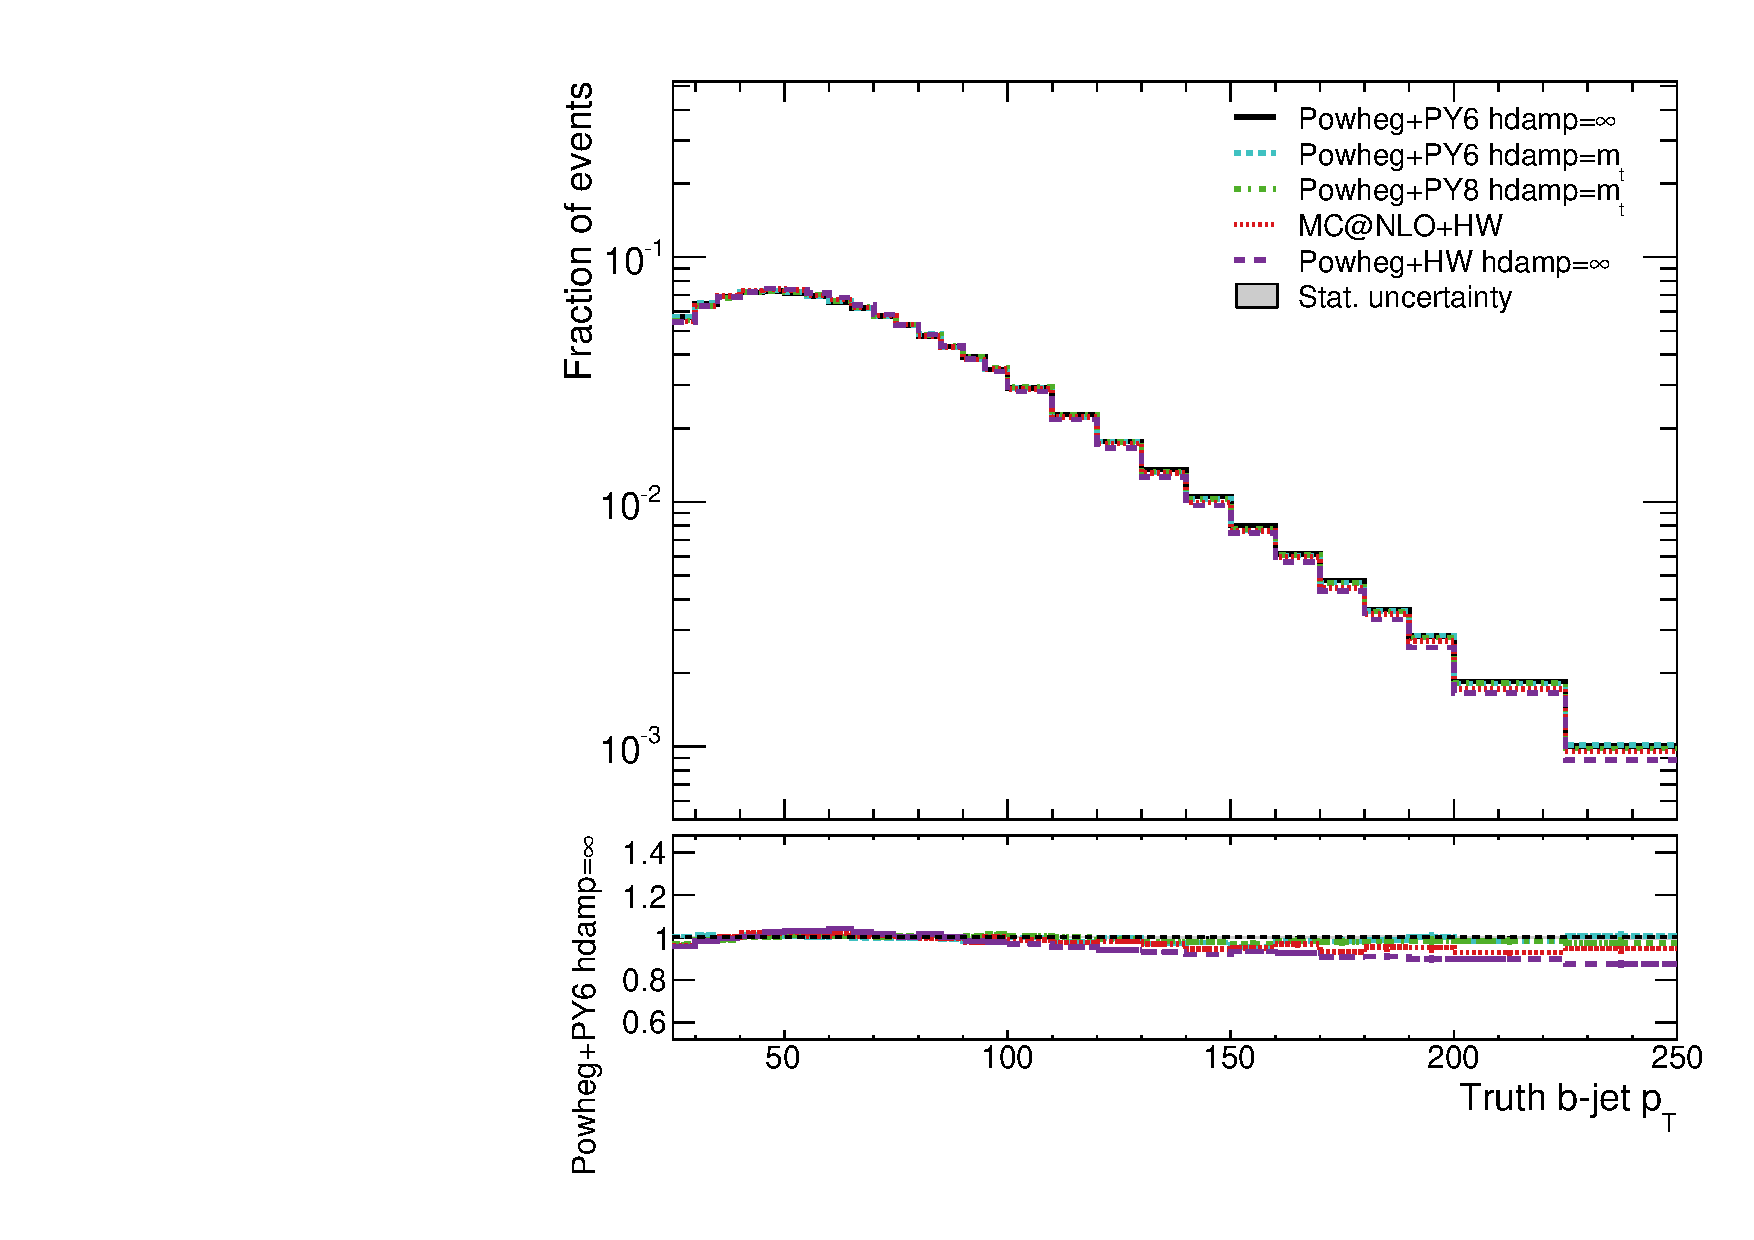
\includegraphics[width=\textwidth]{fig/MCComp/NLO/TruthBJetPt.pdf}
\end{subfigure}
\begin{subfigure}[]{0.45\textwidth}
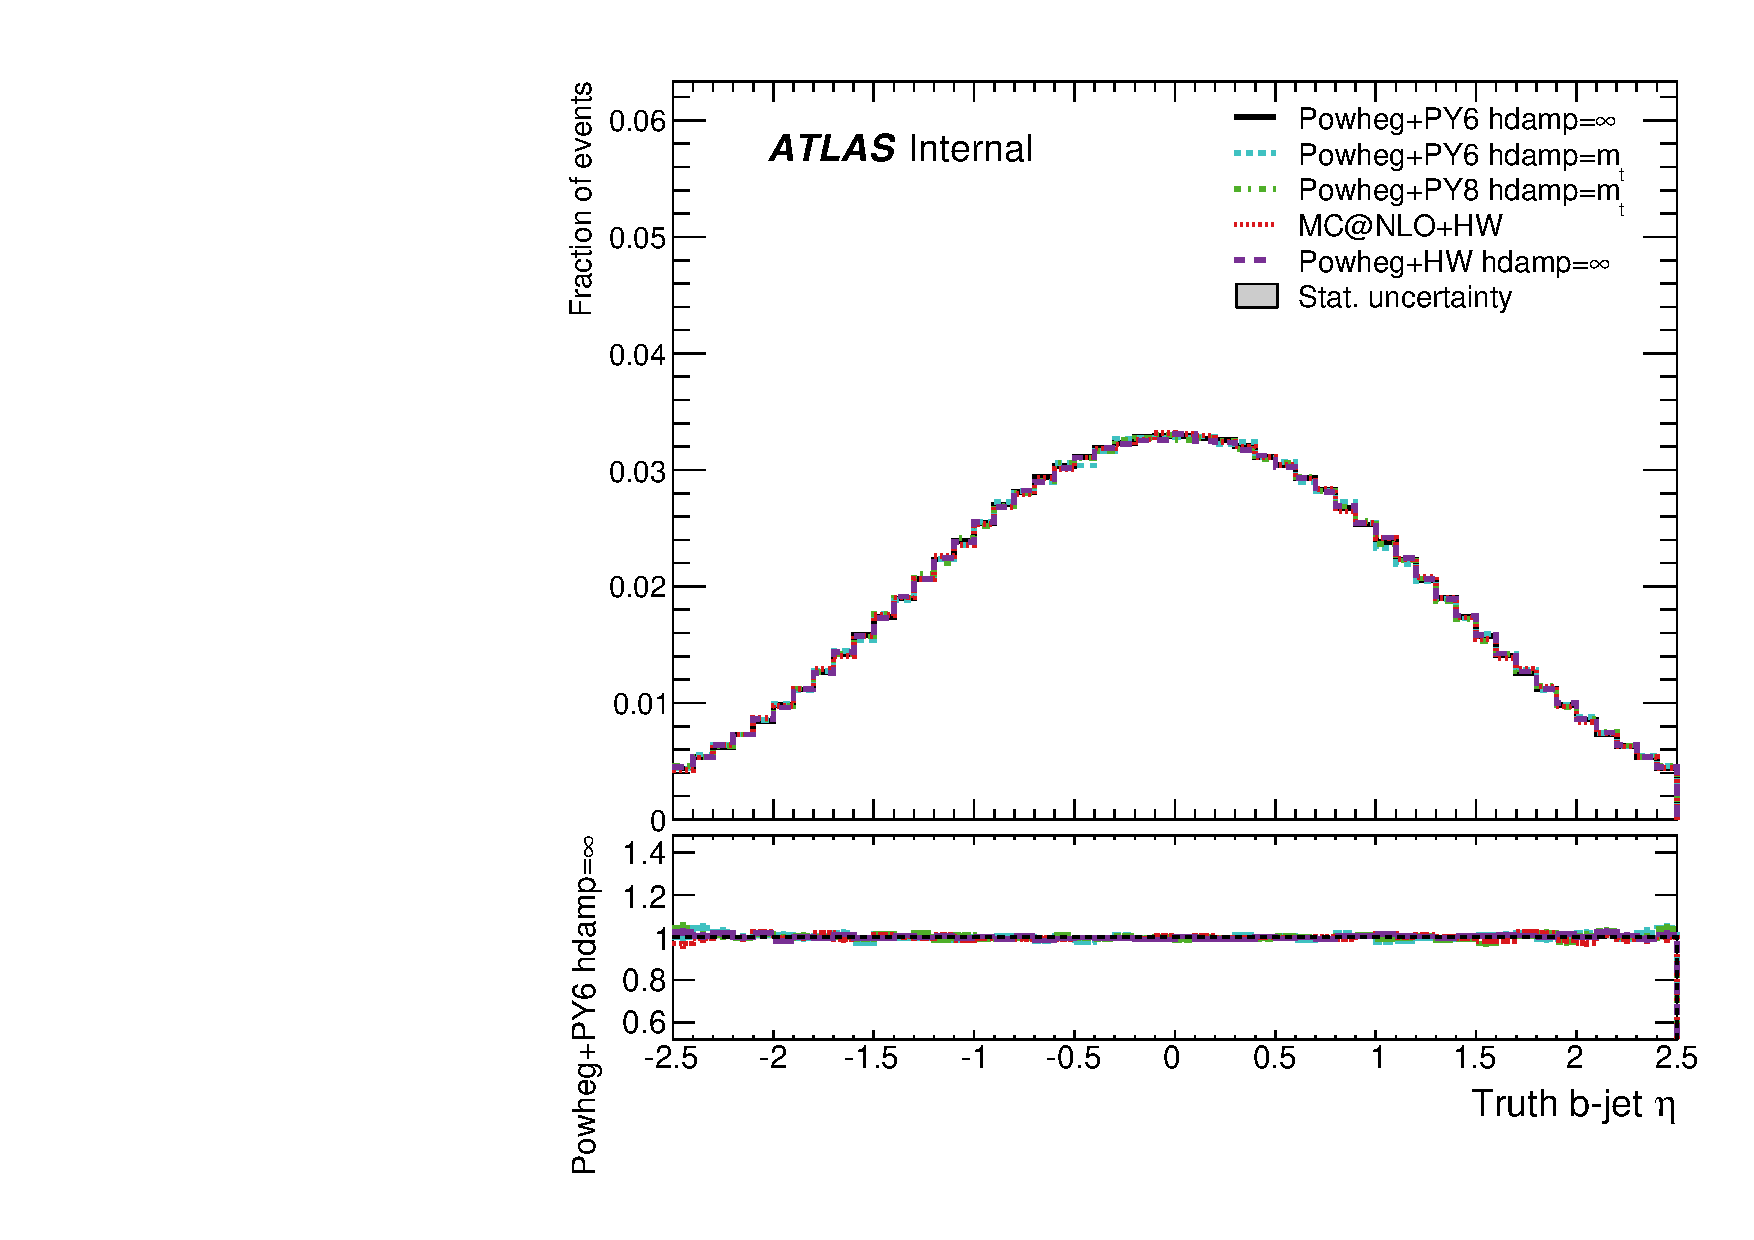
\includegraphics[width=\textwidth]{fig/MCComp/NLO/TruthBJetEta.pdf}
\end{subfigure}
\begin{subfigure}[]{0.45\textwidth}
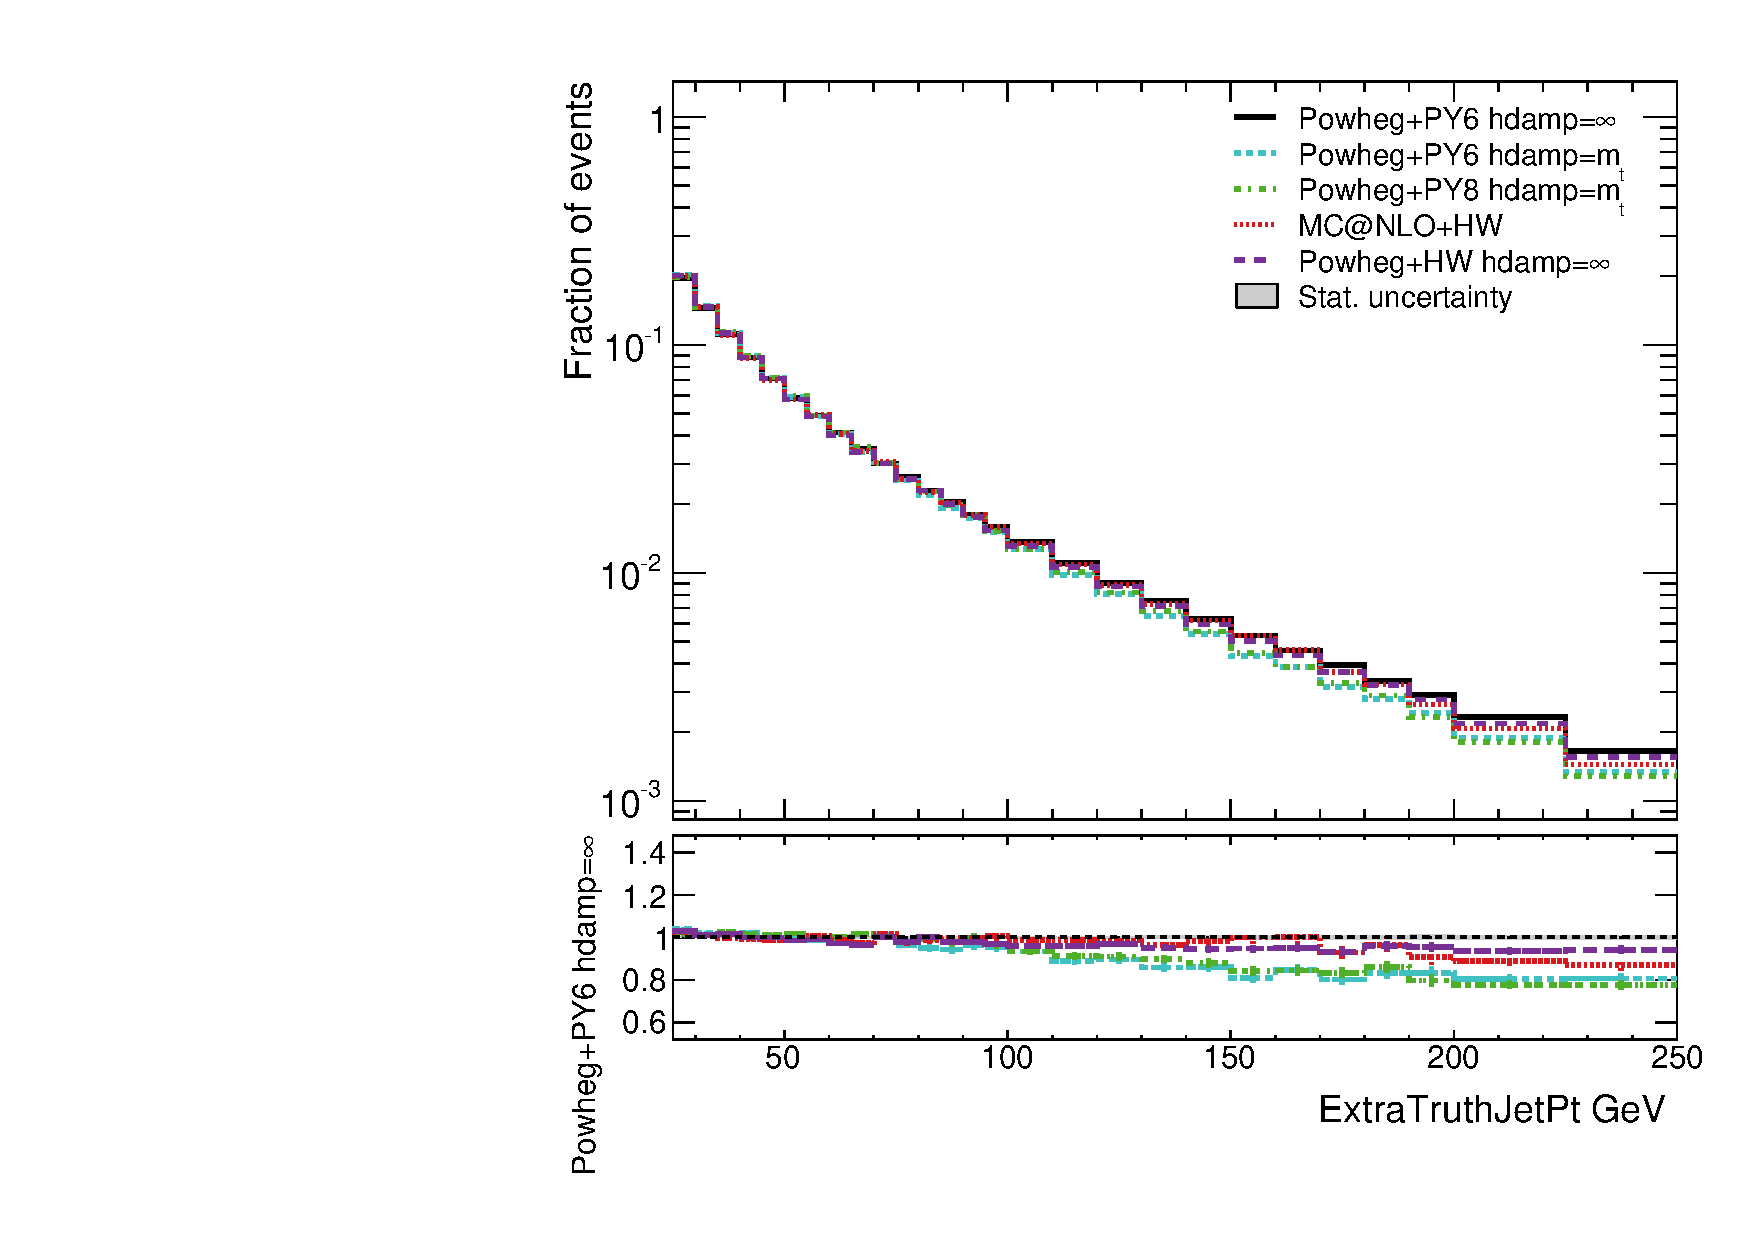
\includegraphics[width=\textwidth]{fig/MCComp/NLO/ExtraTruthJetPt.pdf}
\end{subfigure}
\begin{subfigure}[]{0.45\textwidth}
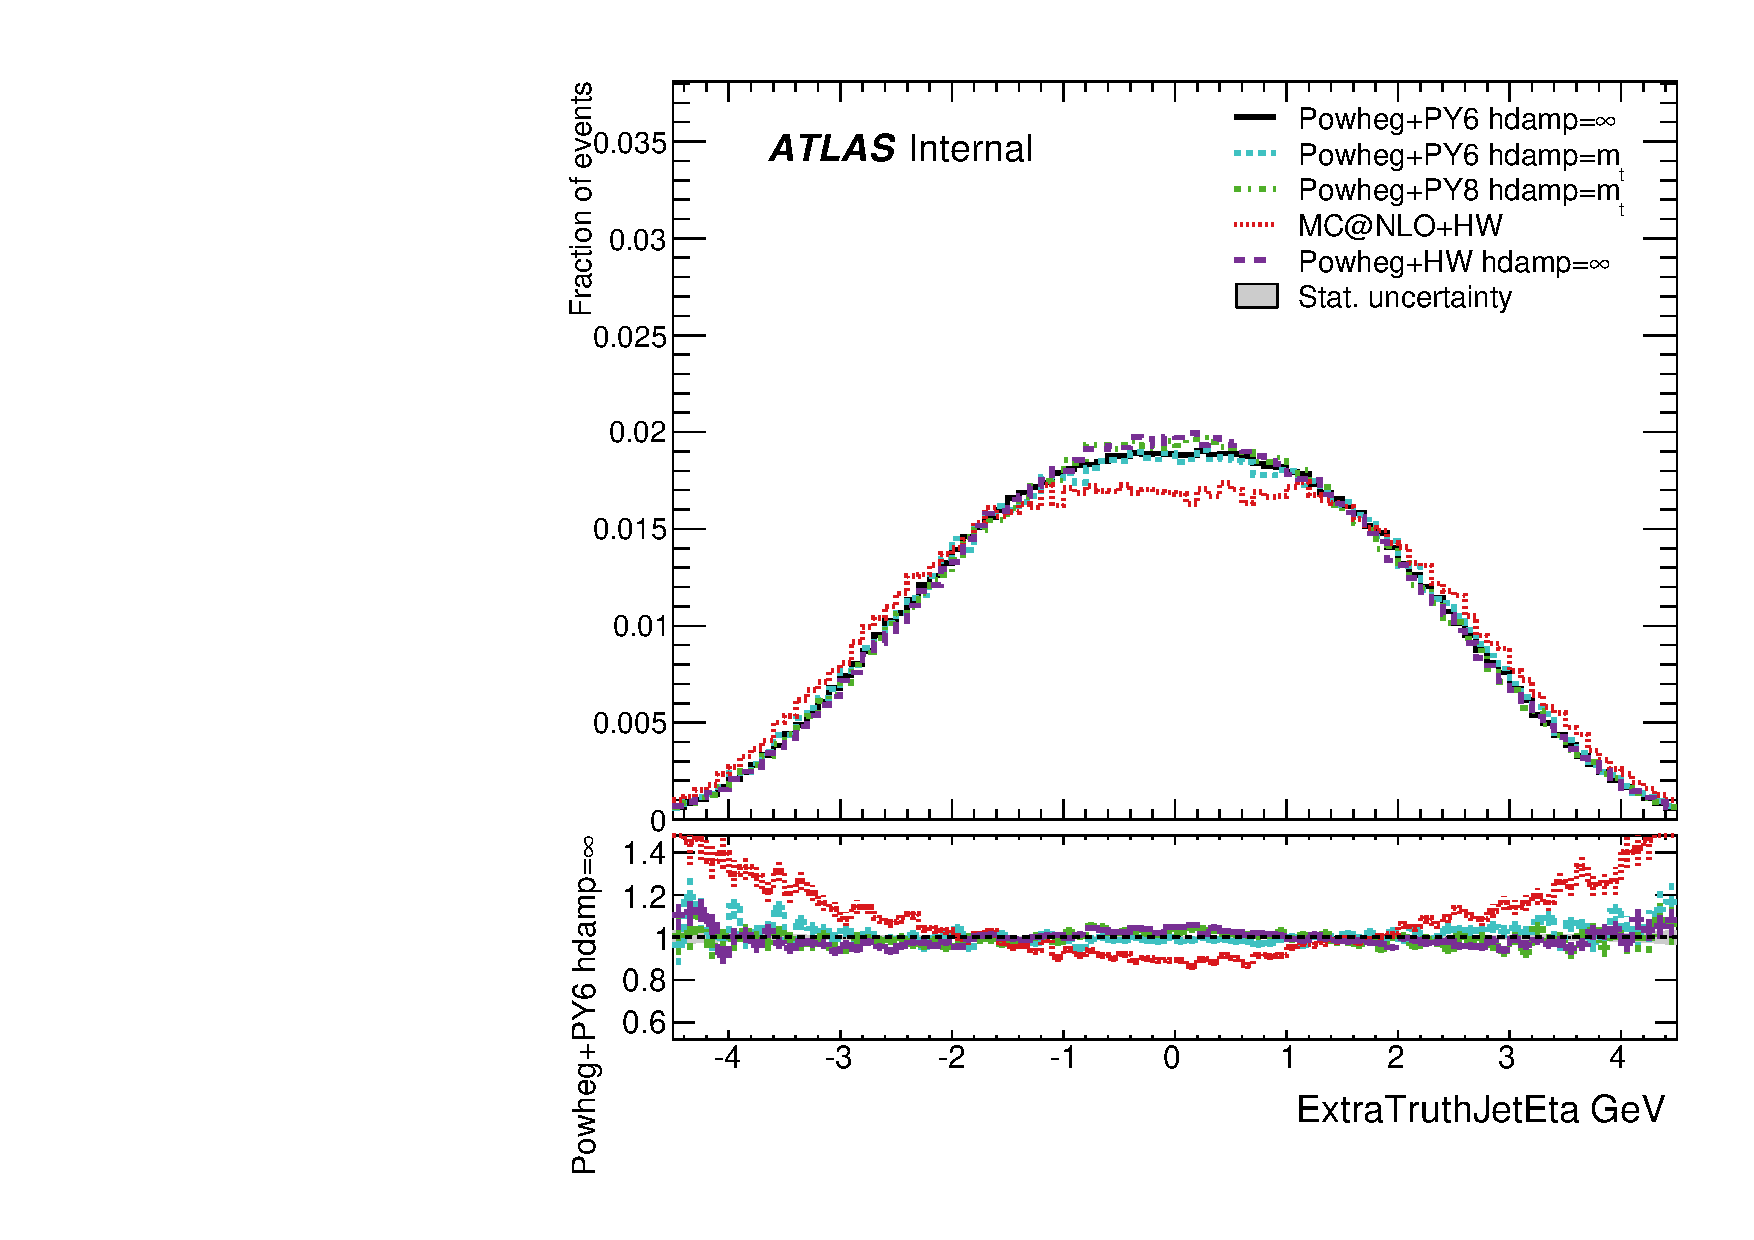
\includegraphics[width=\textwidth]{fig/MCComp/NLO/ExtraTruthJetEta.pdf}
\end{subfigure}
\caption{Distributions of the truth $b$-jet (a) \pt, (b) $b$-jet $\eta$, (c) extra jet  \pt, and (d) extra jet $\eta$ in \ttbar simulation.Several alternate physics models are compared to the baseline, each normalized by the number of selected truth events.}
\label{fig:truthbjet}
\end{figure}
%\clearpage
%\subsection{Extra jets}
\begin{figure}
\centering
\begin{subfigure}[]{0.45\textwidth}
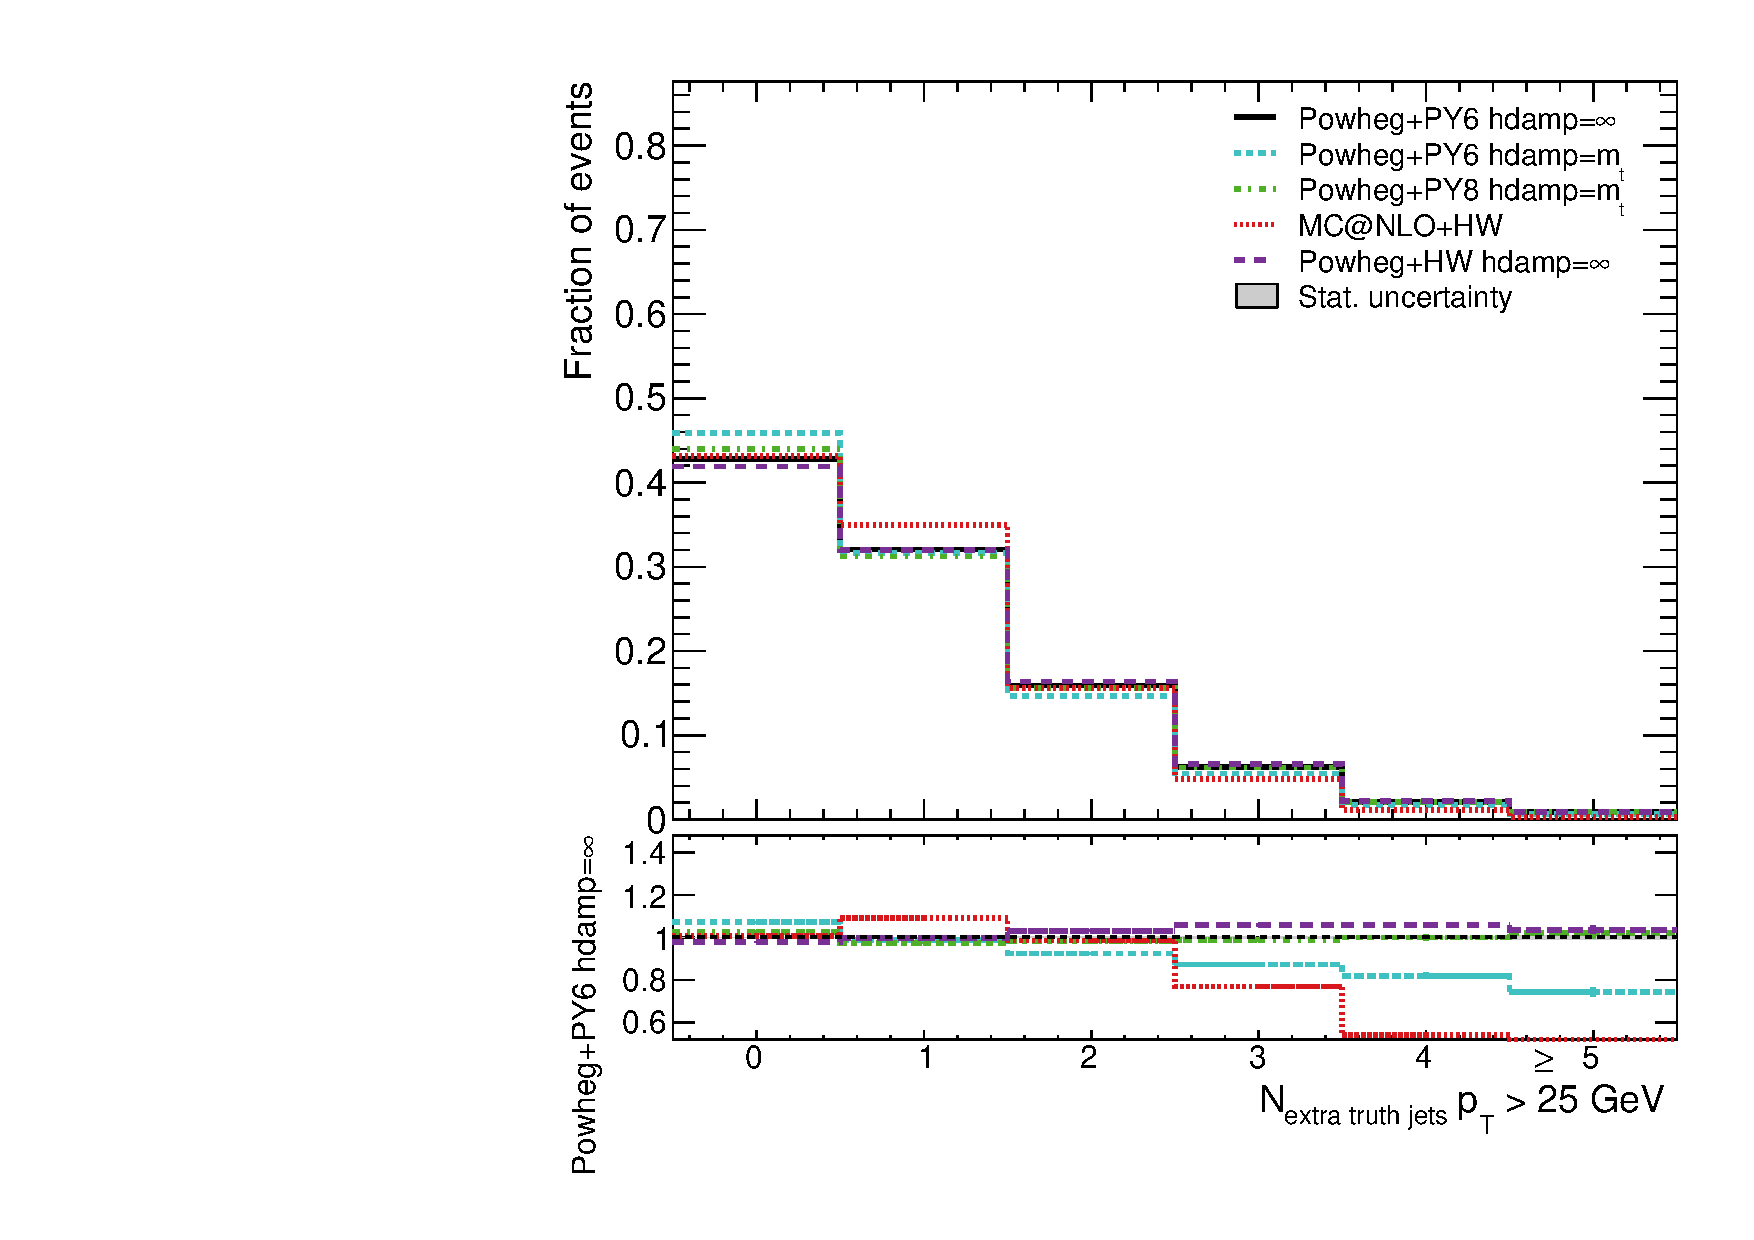
\includegraphics[width=\textwidth]{fig/MCComp/NLO/NTruthExtraJets25.pdf}
\end{subfigure}
\begin{subfigure}[]{0.45\textwidth}
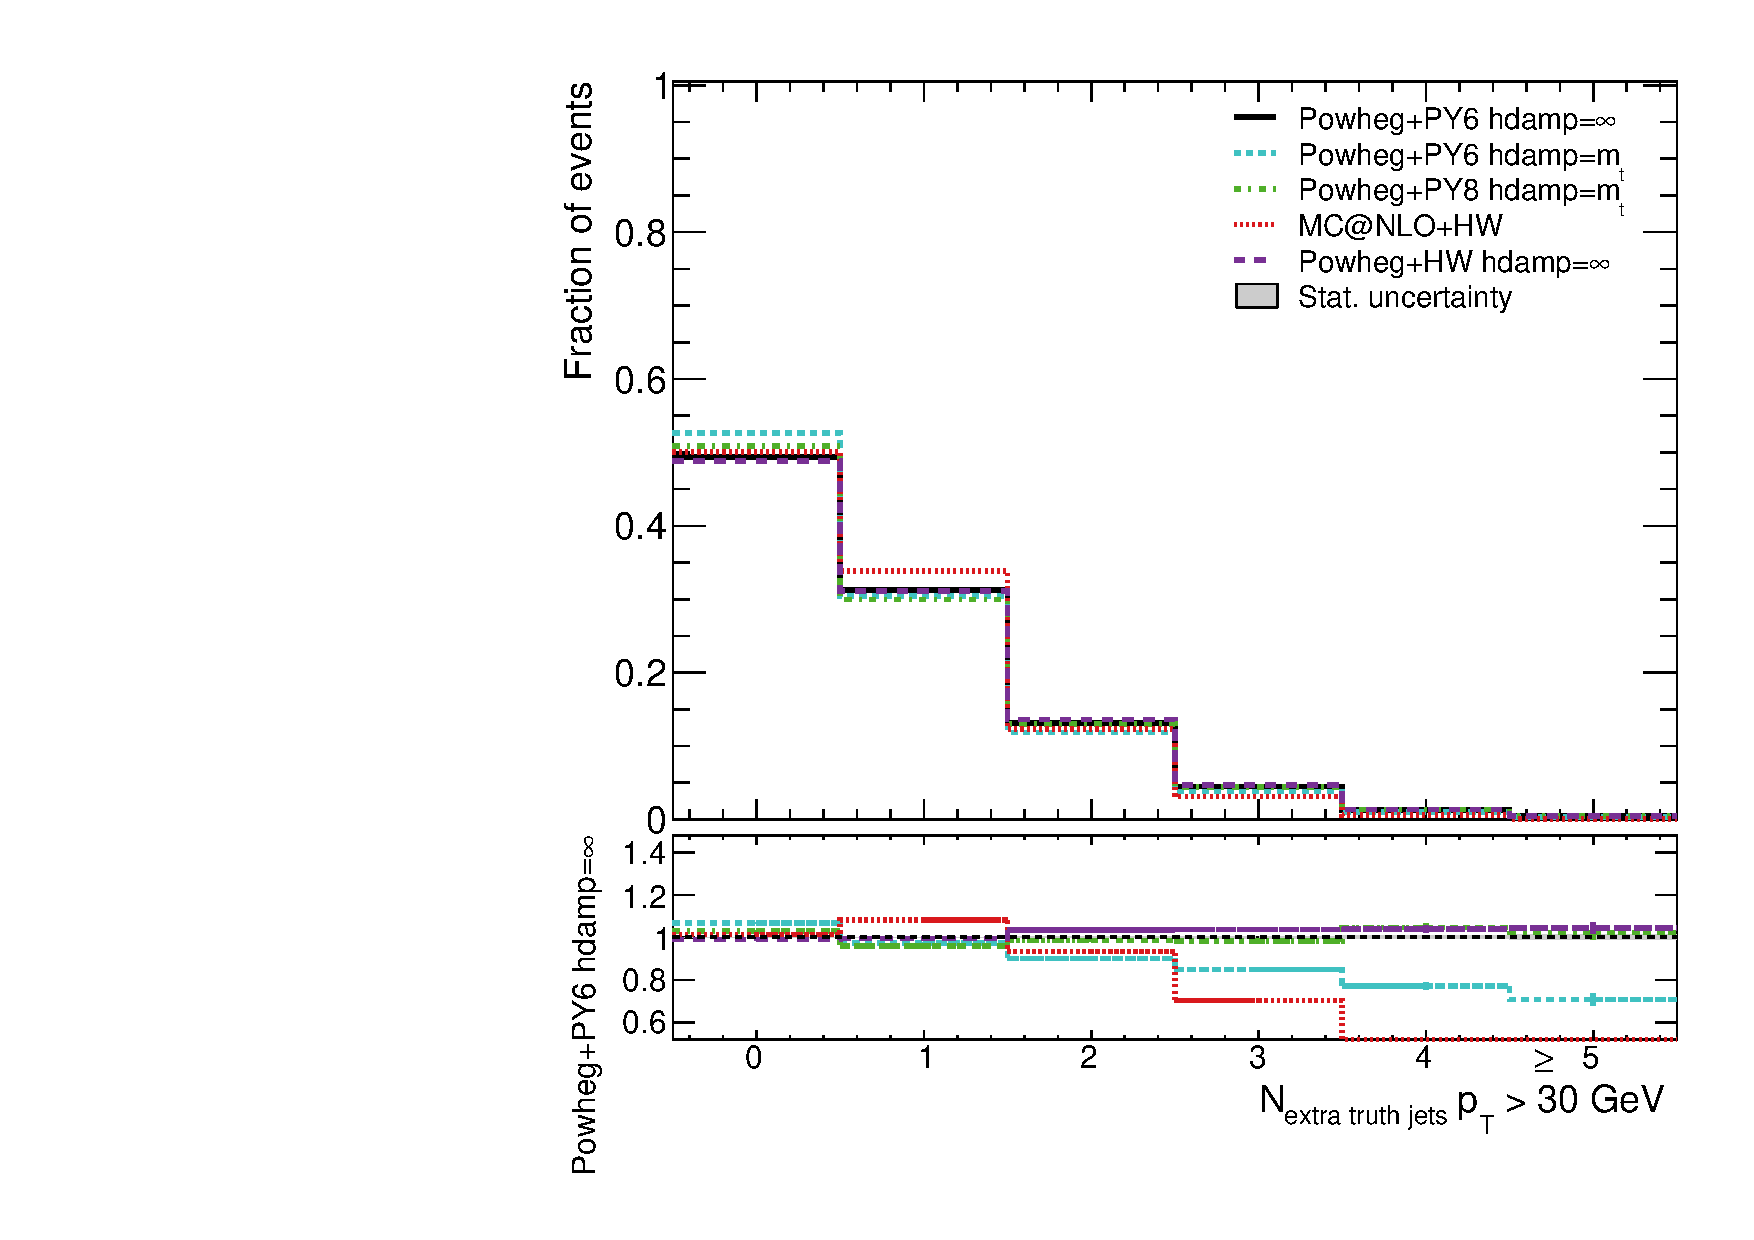
\includegraphics[width=\textwidth]{fig/MCComp/NLO/NTruthExtraJets30.pdf}
\end{subfigure}
\\
\begin{subfigure}[]{0.45\textwidth}
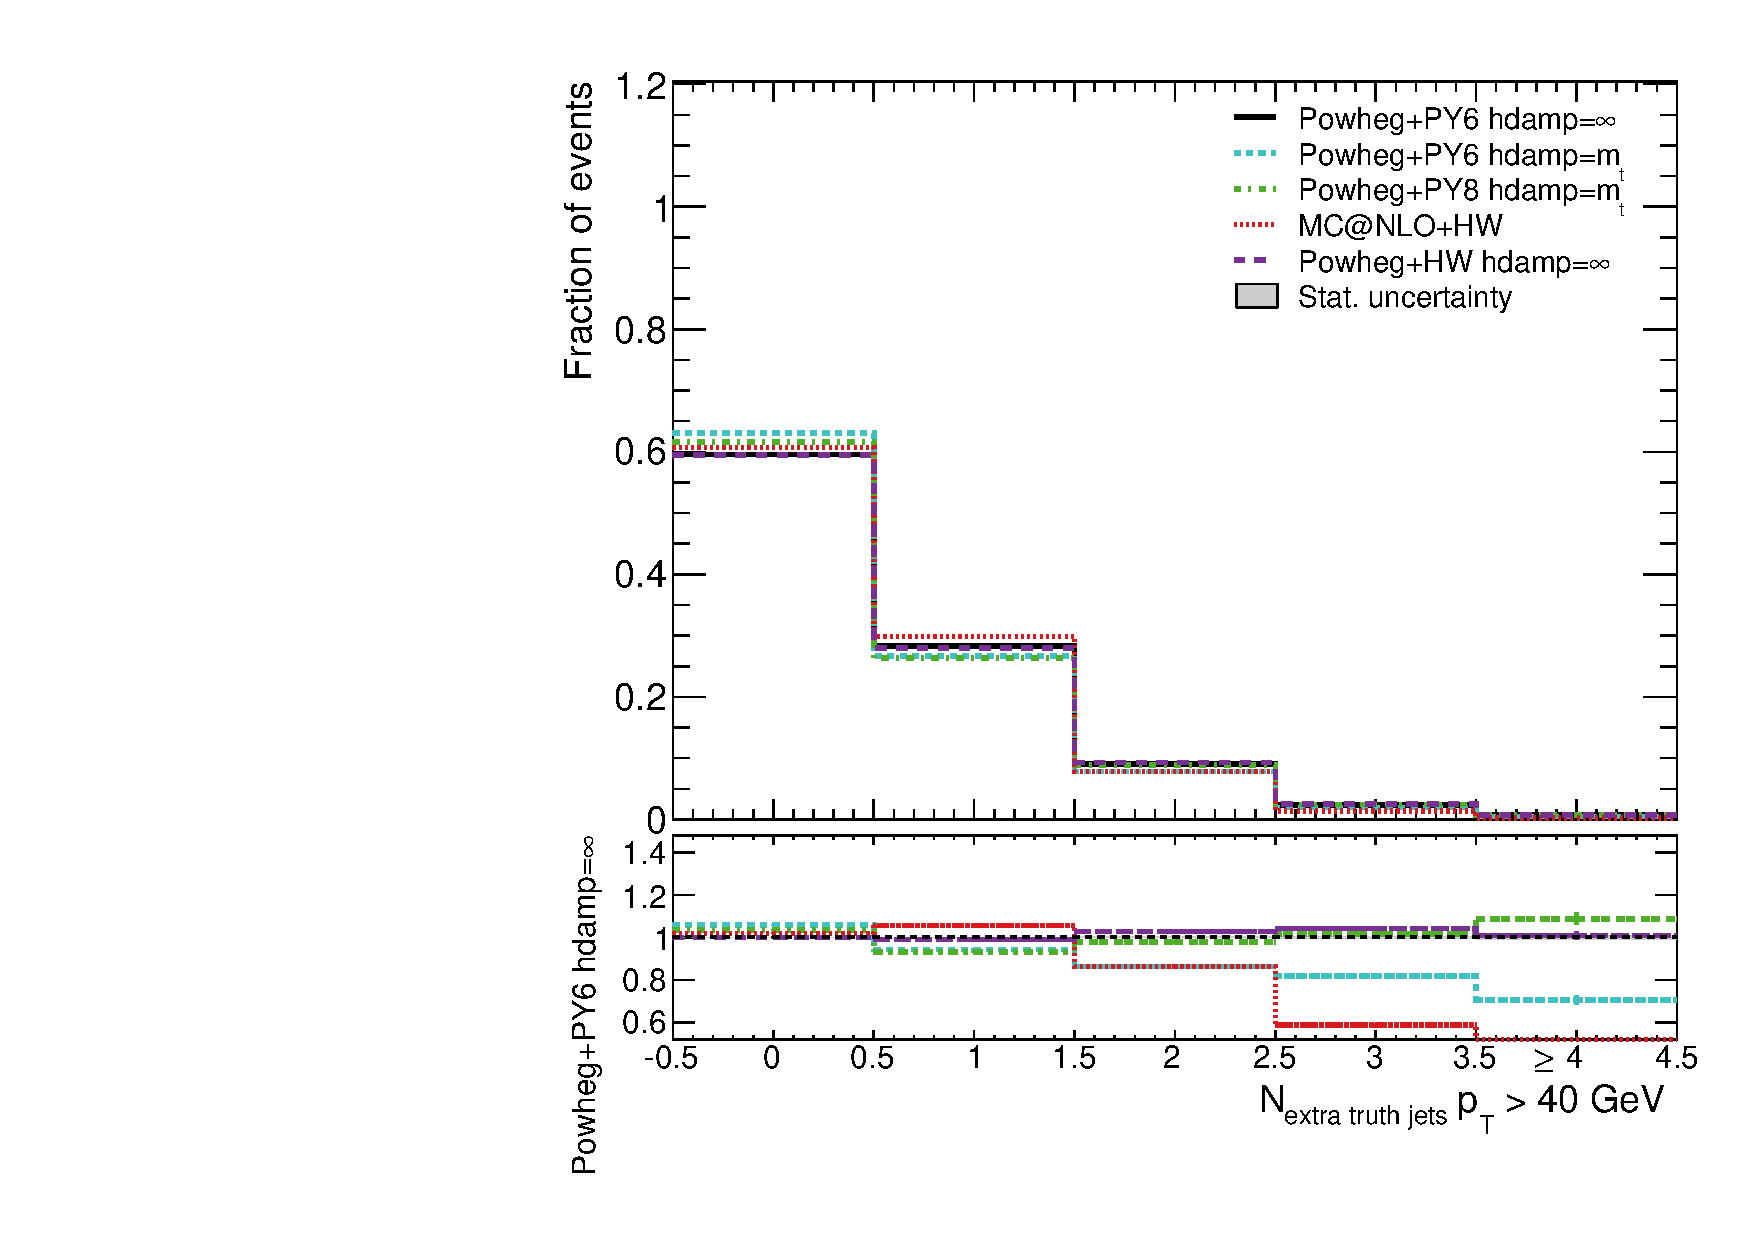
\includegraphics[width=\textwidth]{fig/MCComp/NLO/NTruthExtraJets40.pdf}
\end{subfigure}
\begin{subfigure}[]{0.45\textwidth}
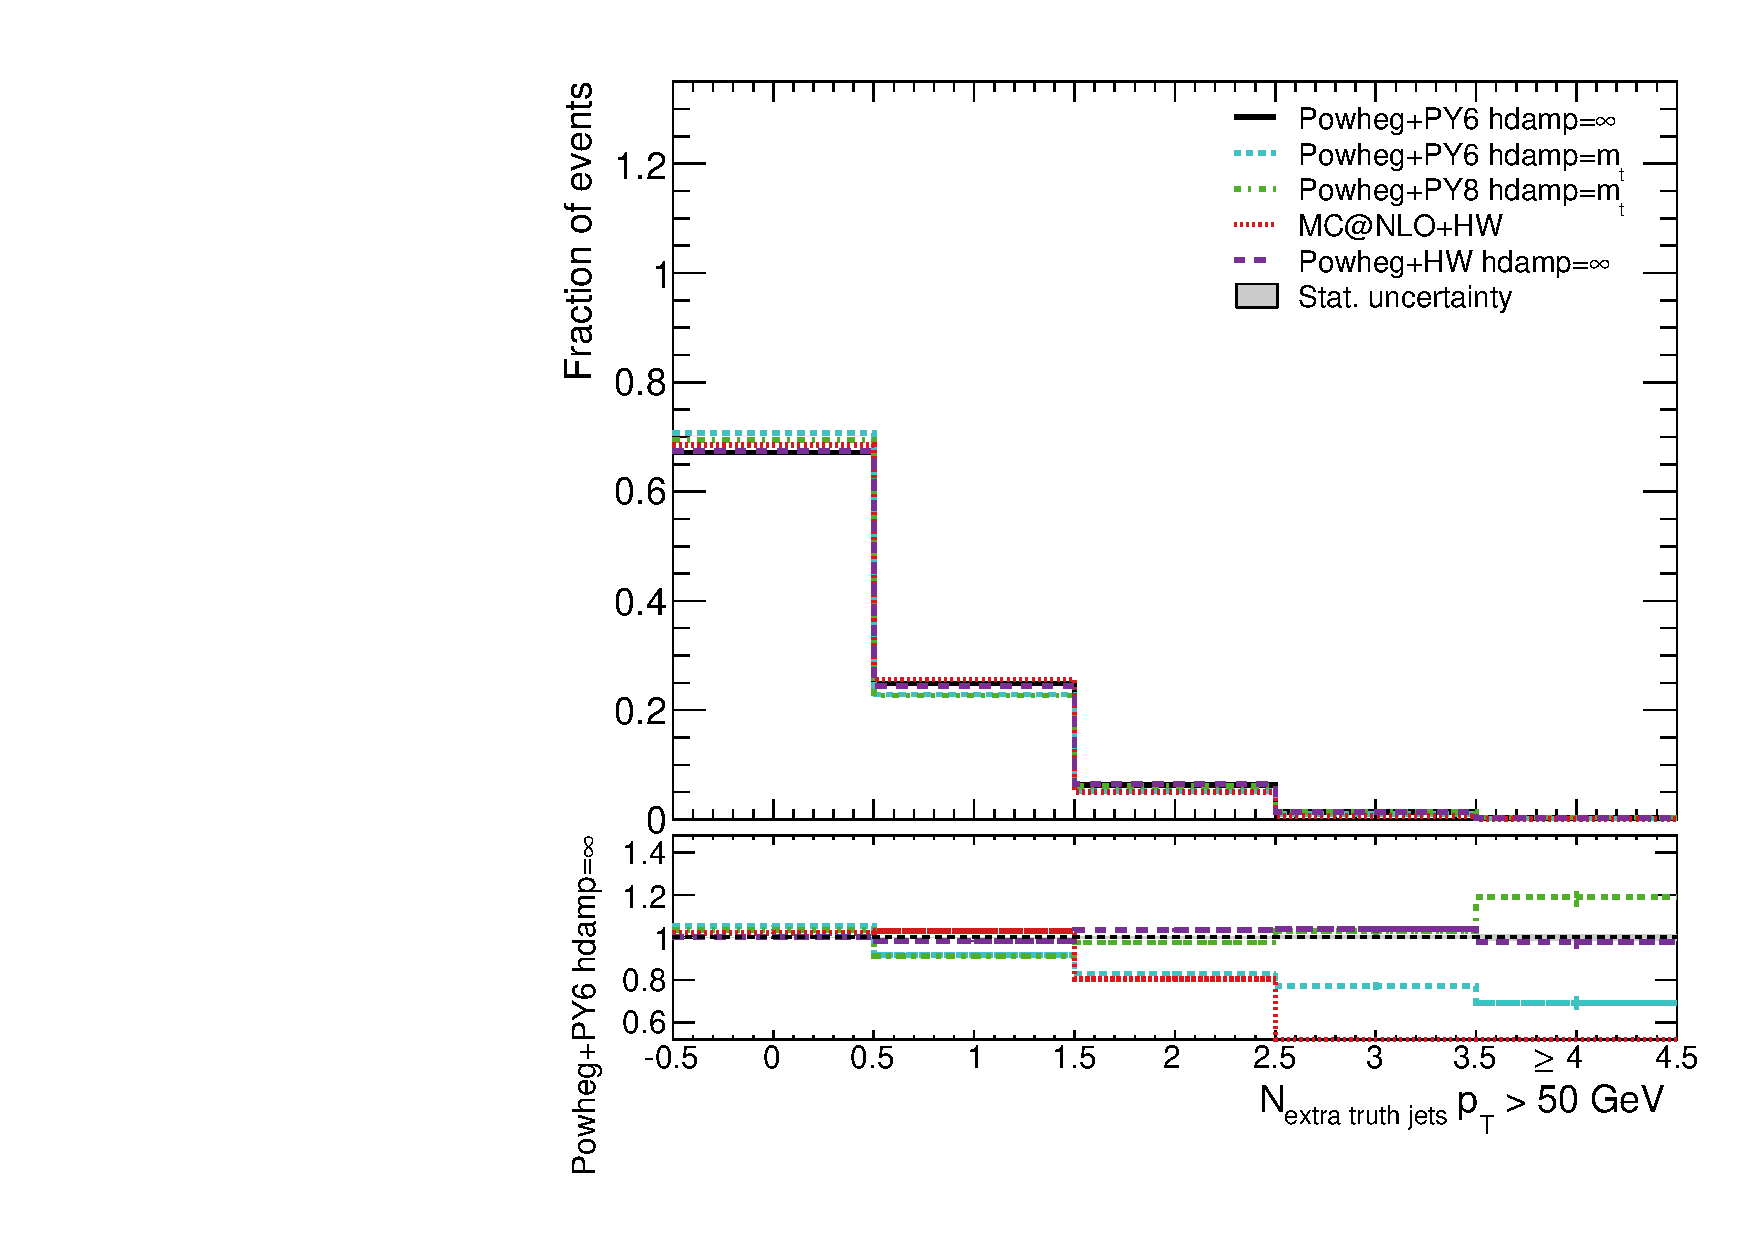
\includegraphics[width=\textwidth]{fig/MCComp/NLO/NTruthExtraJets50.pdf}
\end{subfigure}
\caption{Distributions of the number of extra truth jets with \pt > (a) 25, (b) 30, (c) 40 and (d) 50 \GeV in \ttbar simulation. Several alternate physics models are compared to the baseline, each normalized by the number of selected truth events.}
\label{fig:ntruthjets}
\end{figure}
\begin{figure}
\centering
\begin{subfigure}[]{0.33\textwidth}
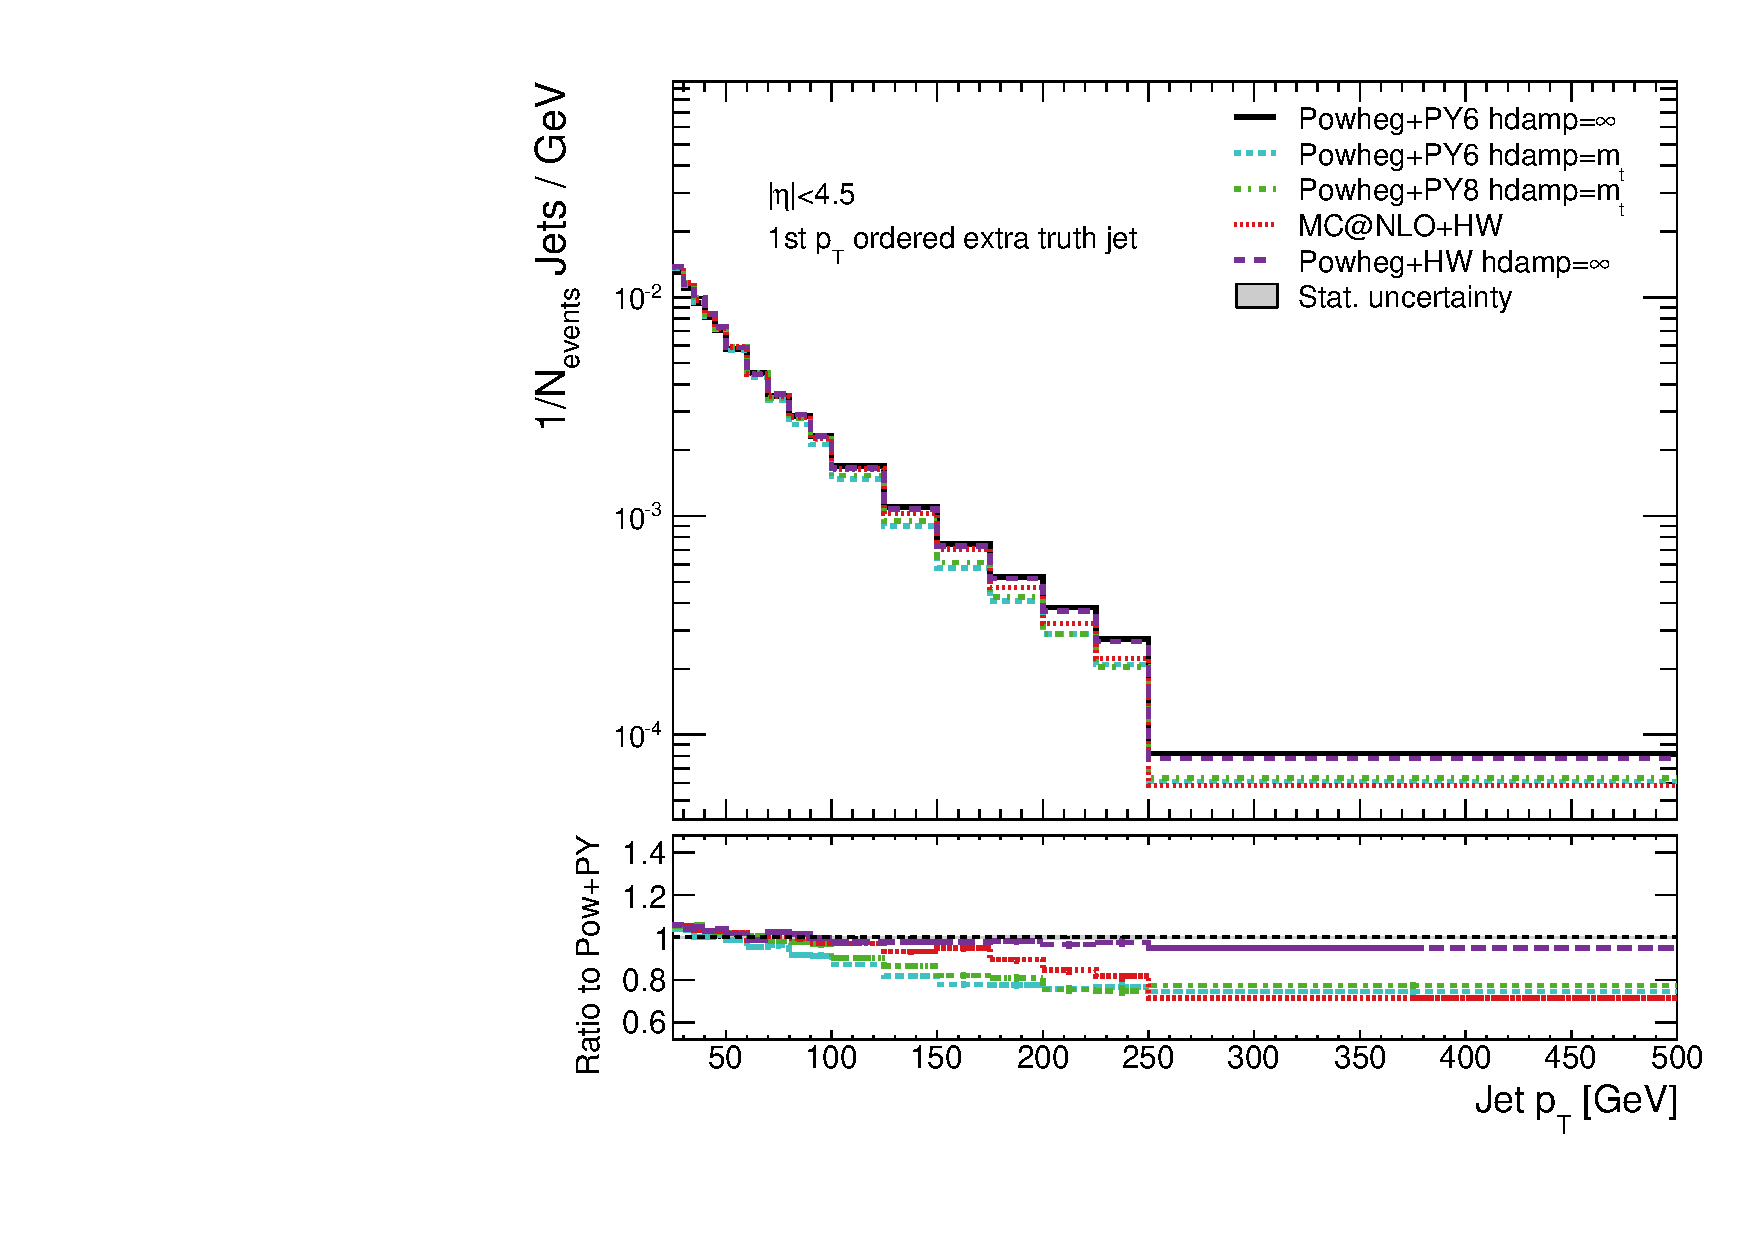
\includegraphics[width=\textwidth]{fig/MCComp/NLO/TruthPtJet0.pdf}
\end{subfigure}
\begin{subfigure}[]{0.33\textwidth}
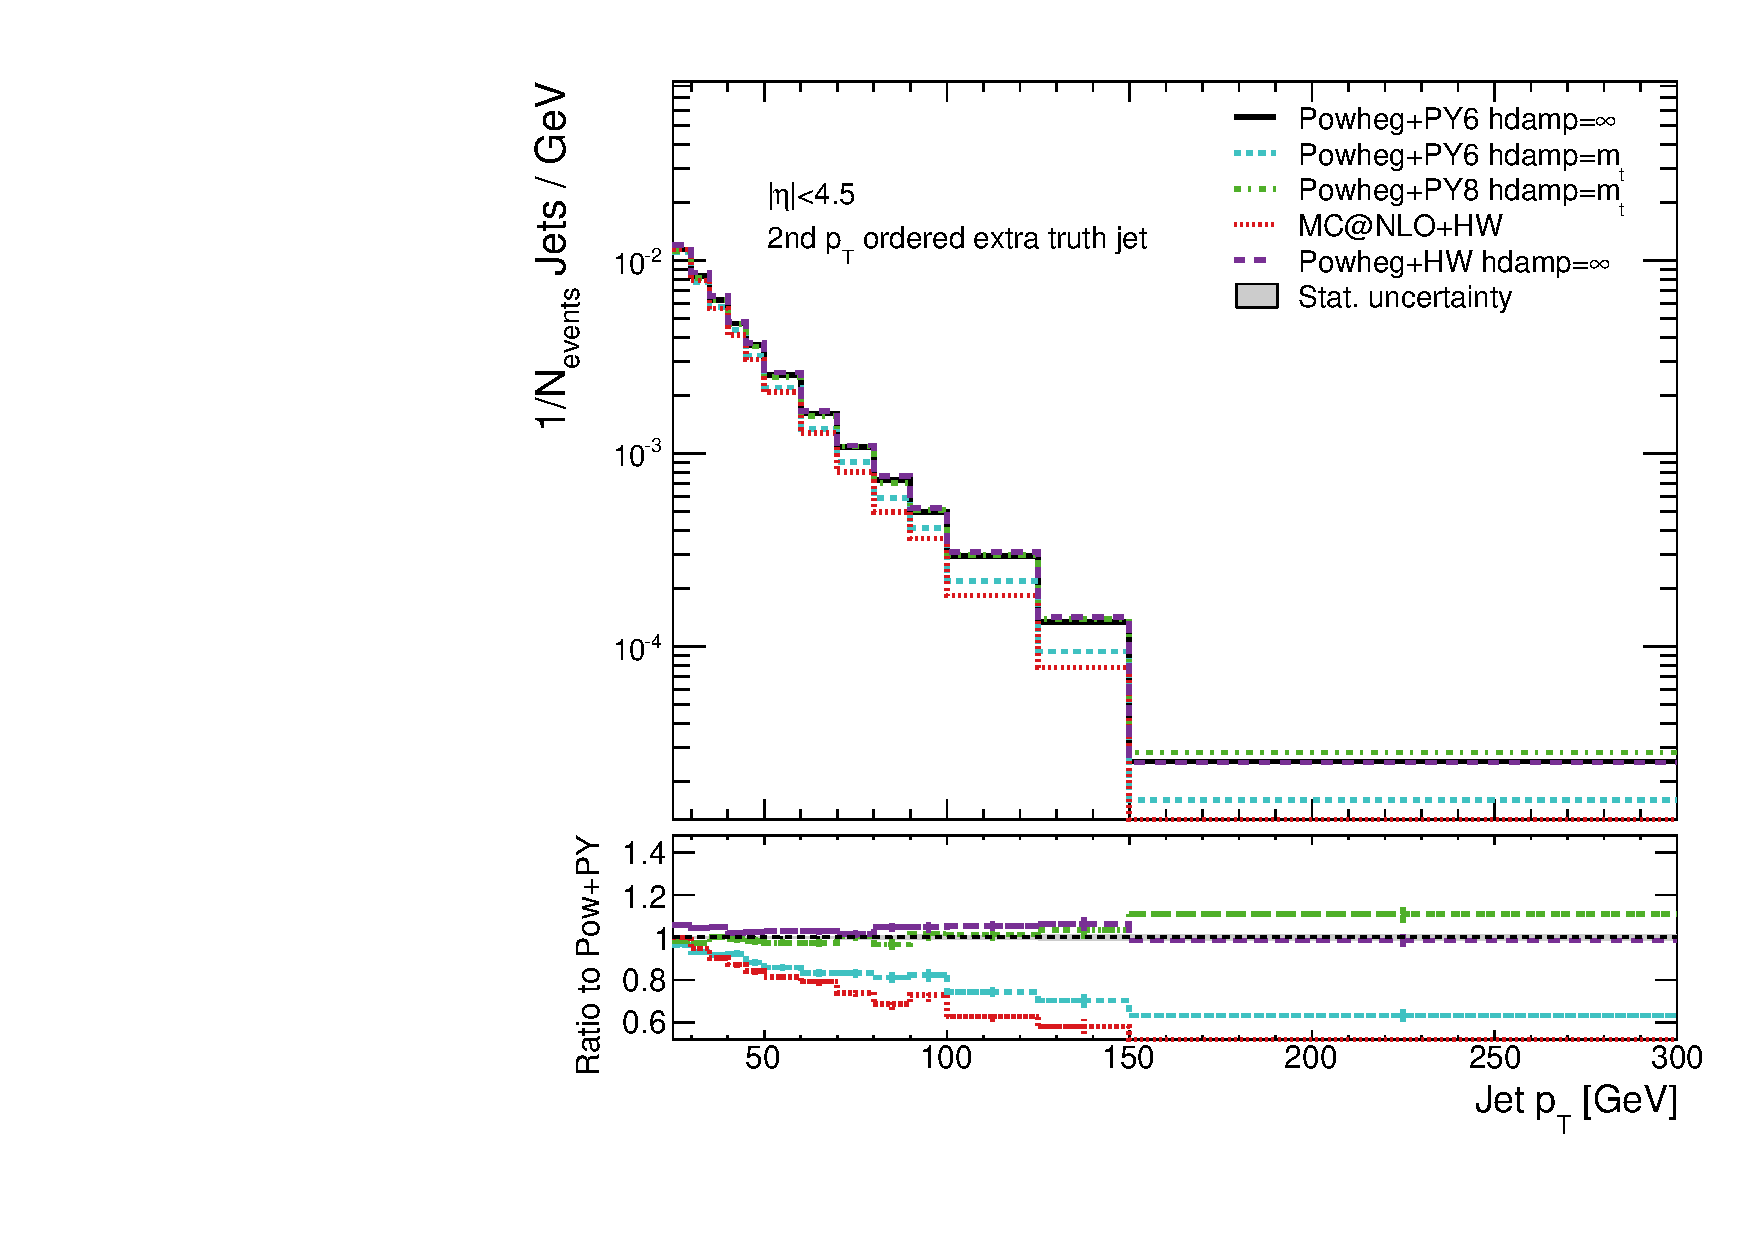
\includegraphics[width=\textwidth]{fig/MCComp/NLO/TruthPtJet1.pdf}
\end{subfigure}
\\
\begin{subfigure}[]{0.33\textwidth}
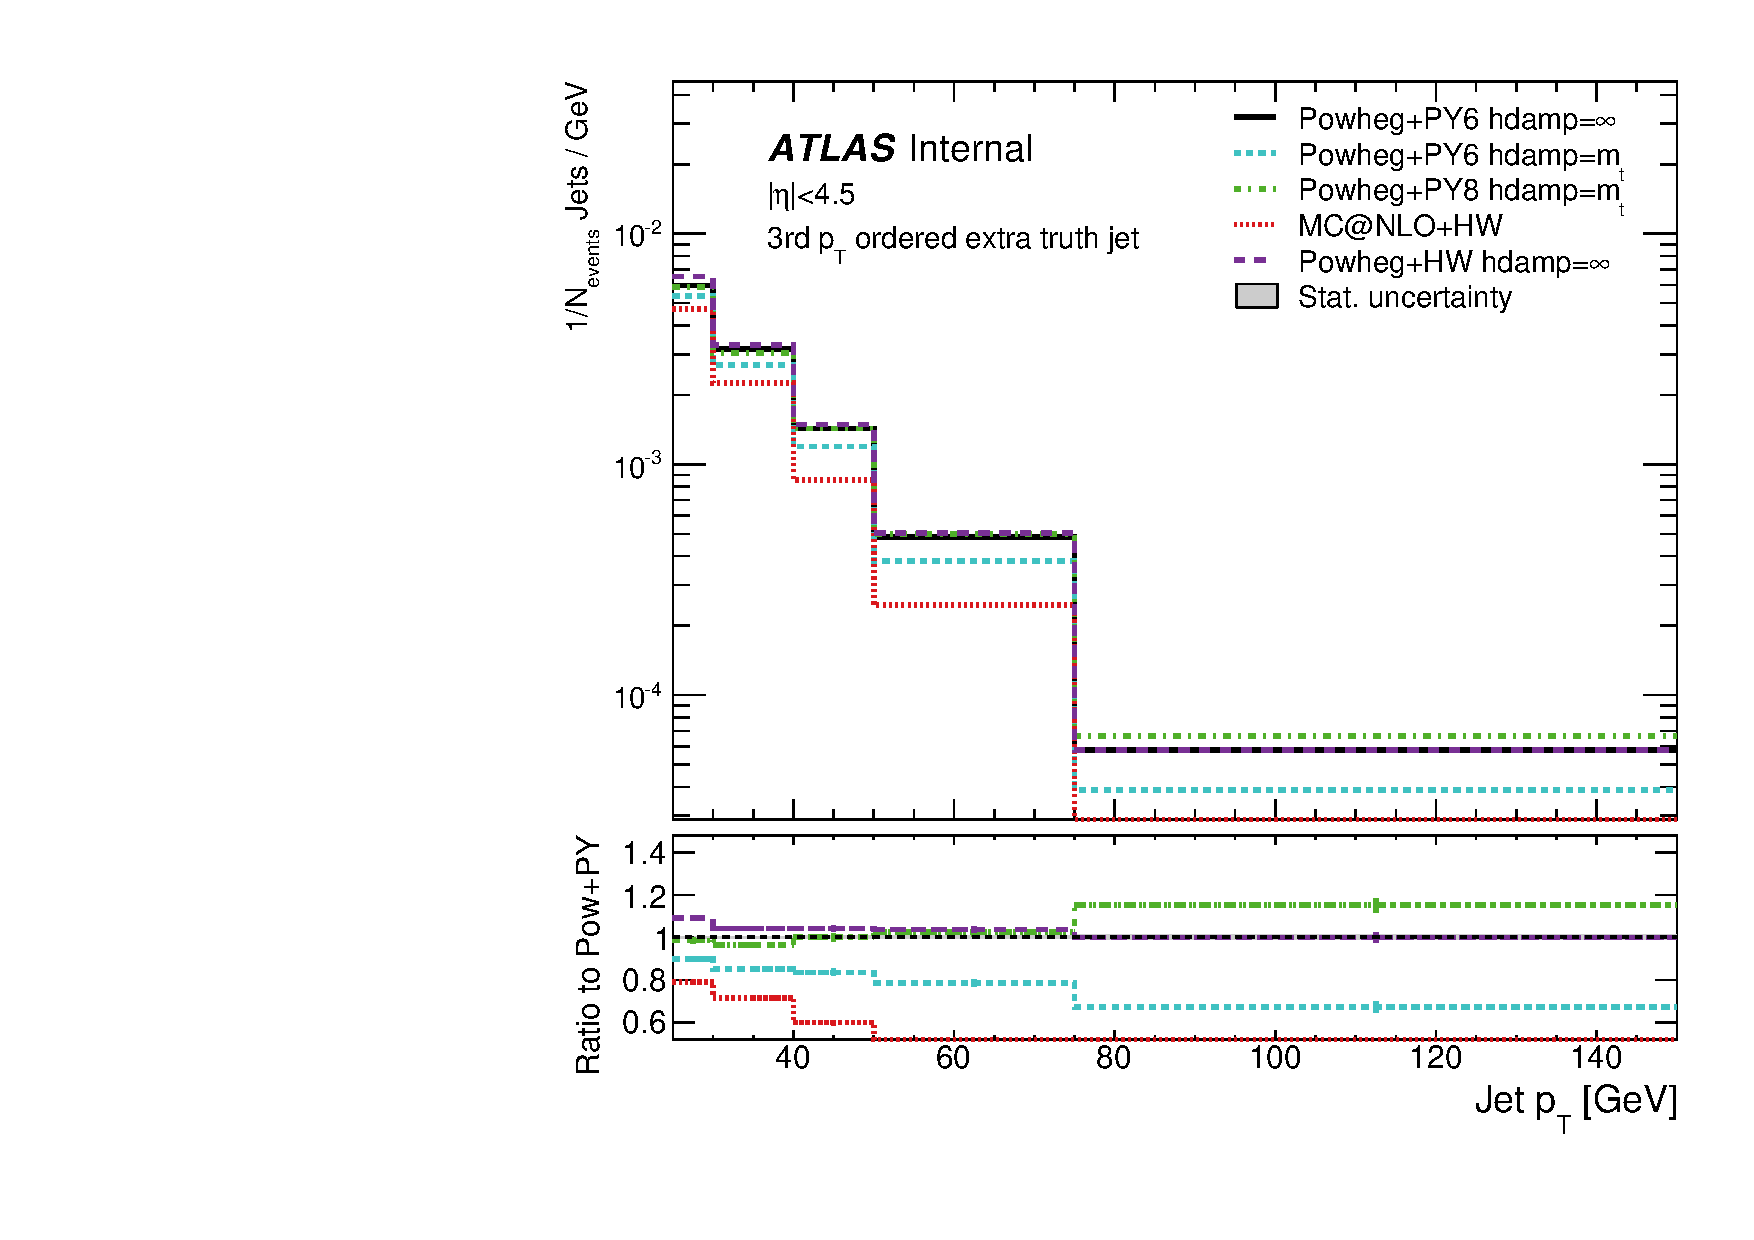
\includegraphics[width=\textwidth]{fig/MCComp/NLO/TruthPtJet2.pdf}
\end{subfigure}
\begin{subfigure}[]{0.33\textwidth}
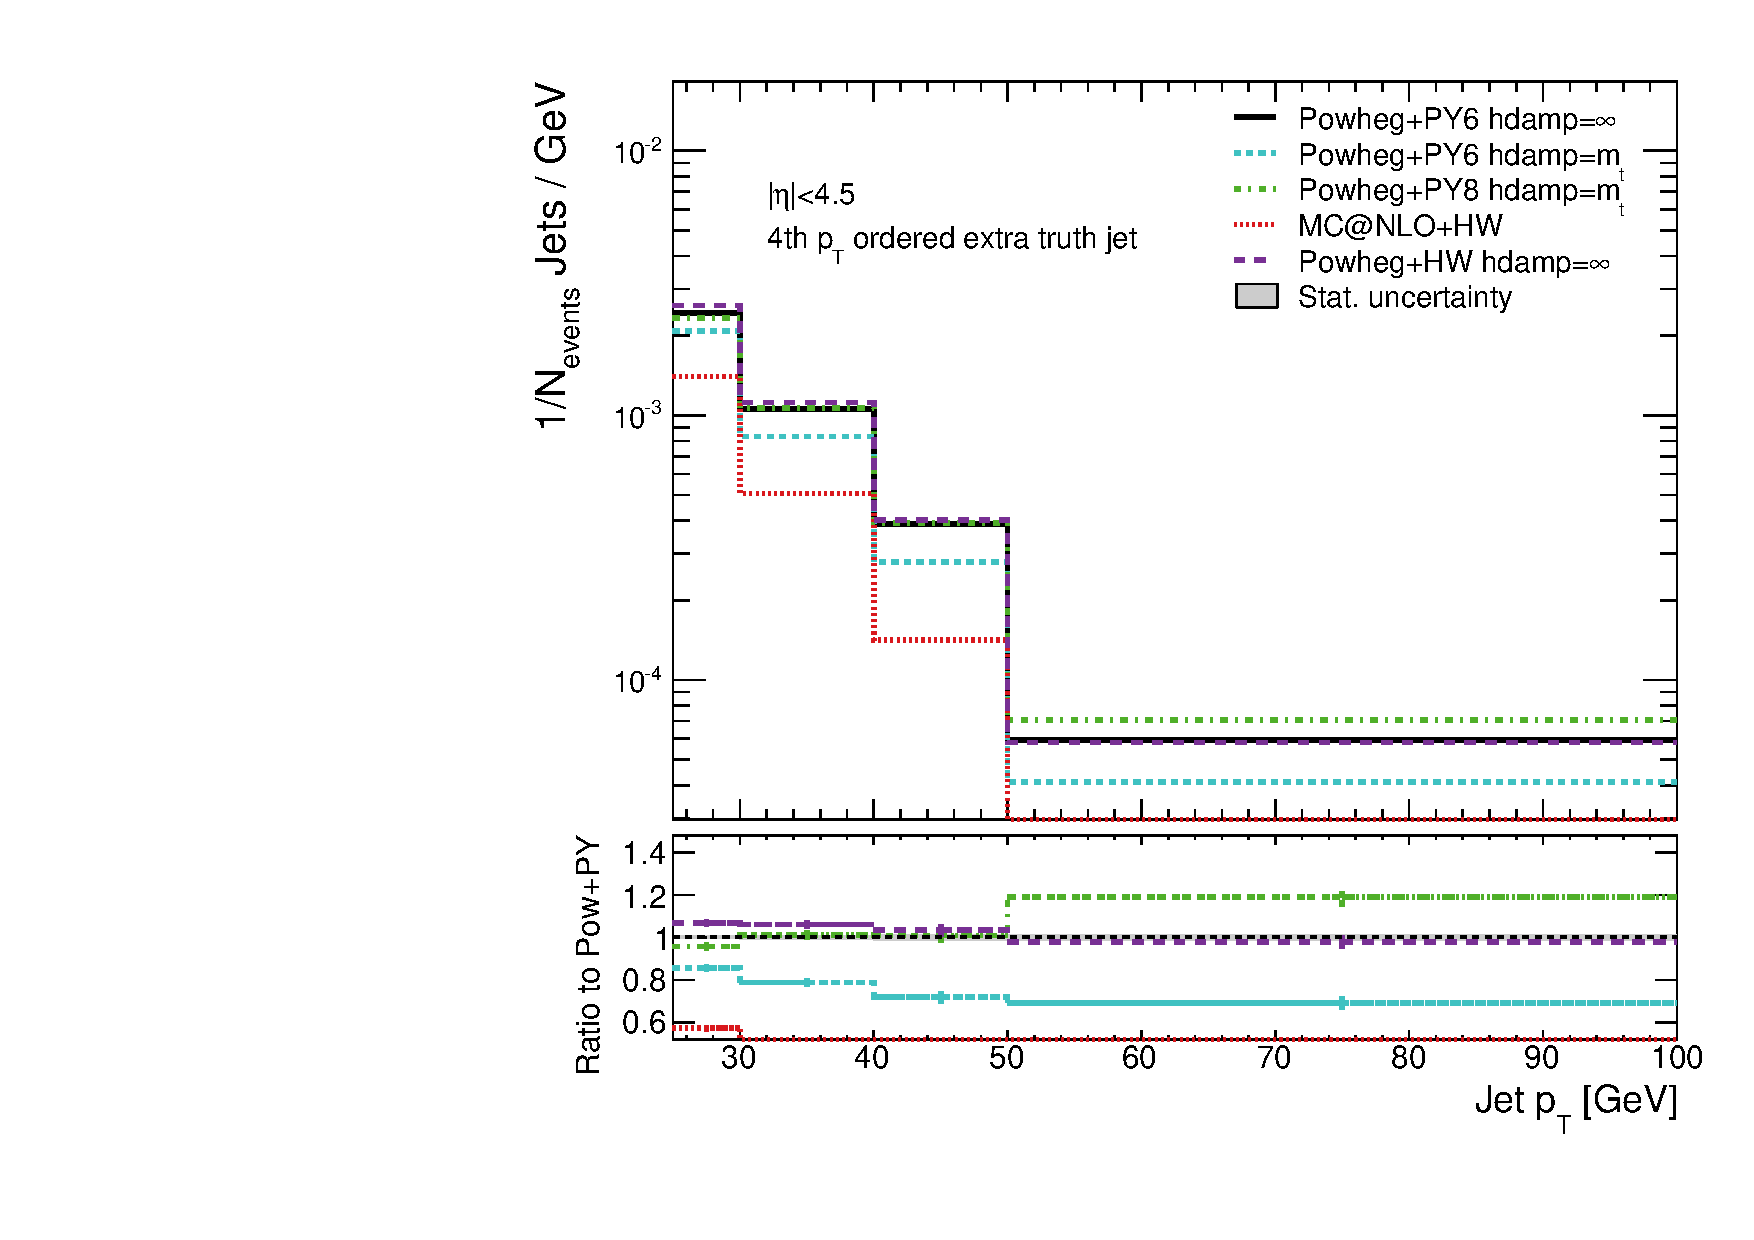
\includegraphics[width=\textwidth]{fig/MCComp/NLO/TruthPtJet3.pdf}
\end{subfigure}
\begin{subfigure}[]{0.33\textwidth}
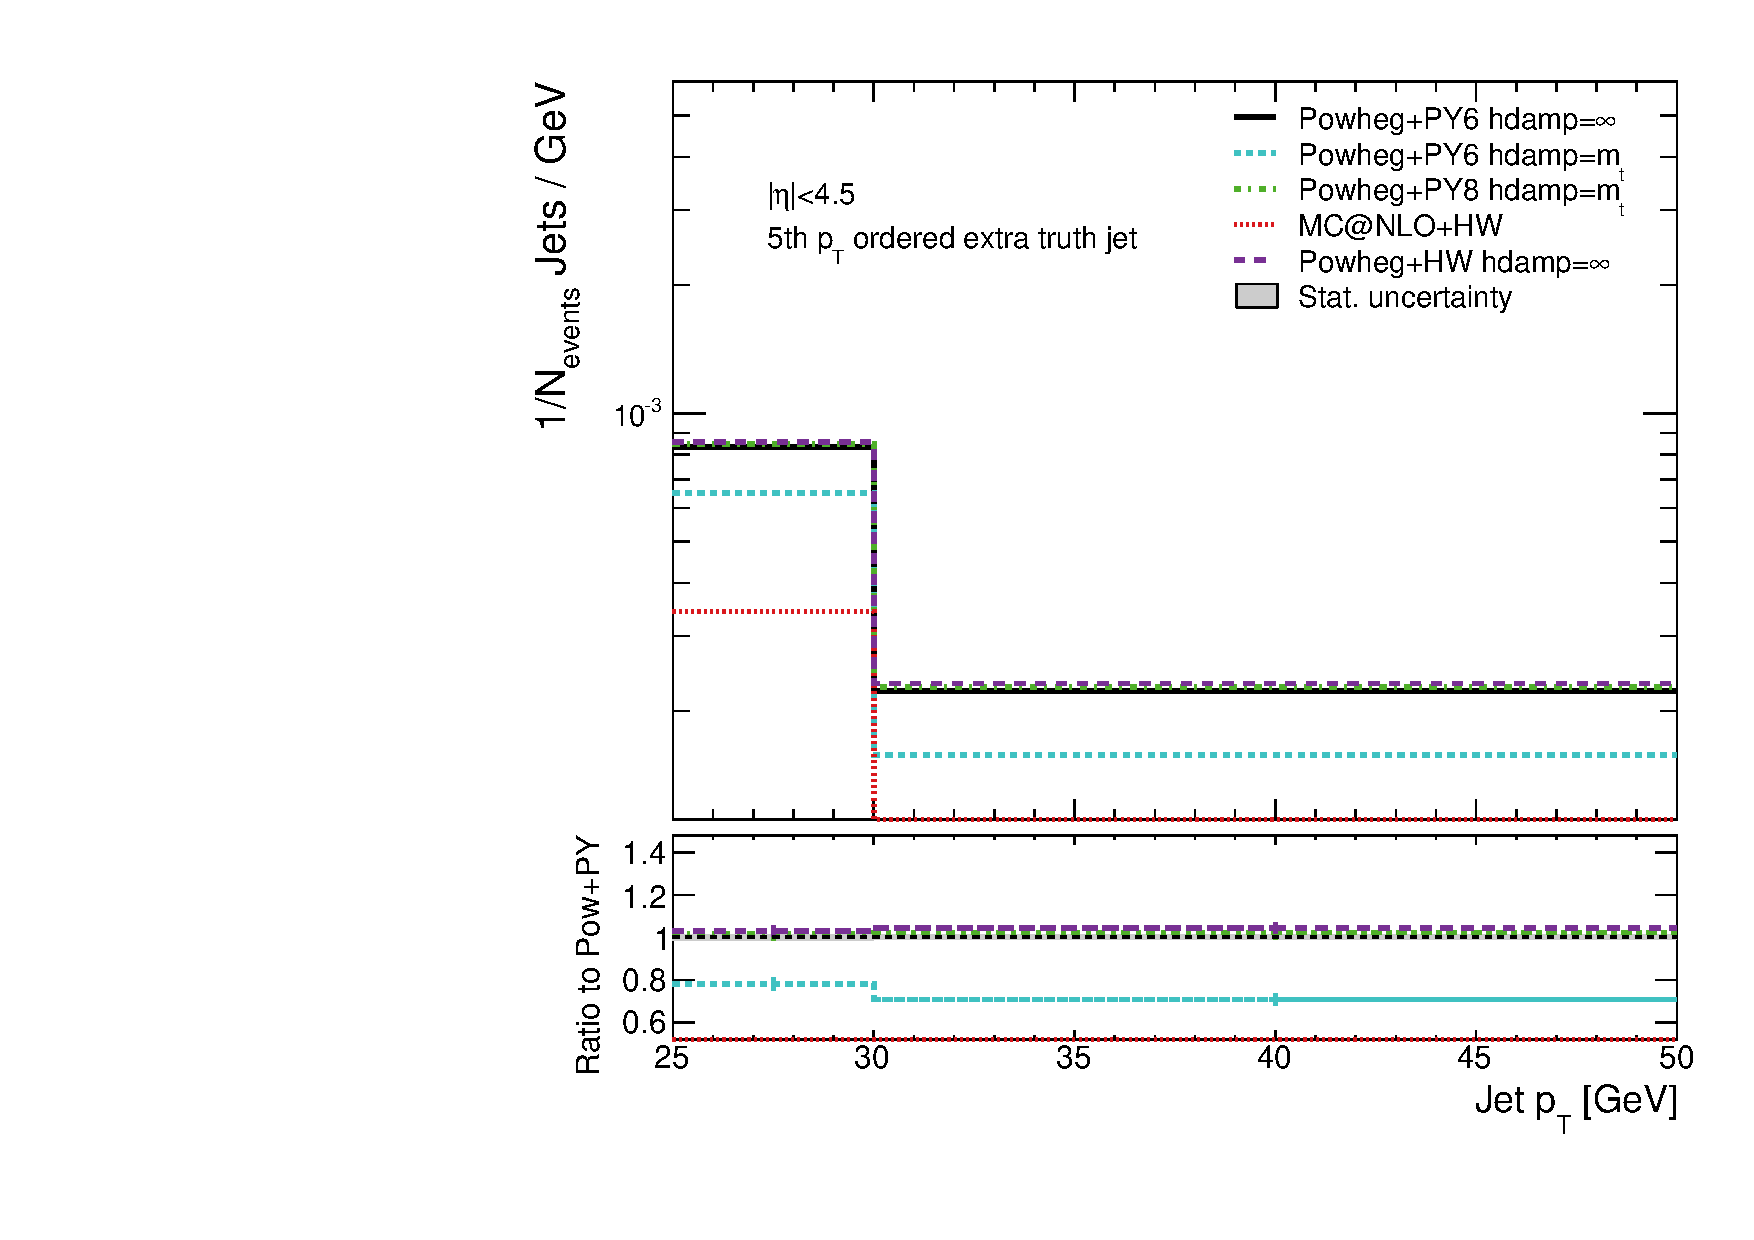
\includegraphics[width=\textwidth]{fig/MCComp/NLO/TruthPtJet4.pdf}
\end{subfigure}
\caption{Distributions of the extra truth jet \pt in \ttbar simulation for jet ranks 1-5 (a-e). Several alternate physics models are compared to the baseline, each normalized by the number of selected truth events.}
\label{fig:truthjetpt}
\end{figure}
%\clearpage
% \subsection{Single top}
% \label{app:truthwt}
% The \ttbar\ final states cannot be distinguished experimentally and at NLO cannot be unambiguously 
% distinguished theoretically.  At present, none of the available NLO generators provide a complete description of
% \emubb\  final state.  It is therefore necessary to compare the measured extra jet distribution to the
% sum of the predictions for the \ttbar\ and $Wt$ processes, where process is weighted by its respective cross section.
% As a result, the uncertainty in the prediction depends on the theoretical uncertainty on the $Wt$ production cross section
% and on the degree to which the extra jet kinematic distributions differ between the \ttbar\ and $Wt$ samples.
% Figures~\ref{fig:wtntruthjets} and~\ref{fig:wttruthjetpt} compare the extra multiplicity and transverse momentum
% distributions of the baseline \ttbar\ sample with those obtained with the three $Wt$ samples used in this analysis 
% ({\sc Powheg+Pythia} diagram removal, {\sc Powheg+Pythia} diagram subtraction and \mcnlohw).  The $Wt$ samples have
% lower extra jet multiplicity and softer extra jet transverse momentum spectra than the \ttbar\ sample.  The level
% of disagreement between the two physics processes is comparable to the observed difference between 
% the {\sc Powheg+Pythia} hdamp=$\infty$ and the {\sc MC@NLO+Herwig} \ttbar\ samples.

% \begin{figure}
% \centering
% \begin{subfigure}[]{0.45\textwidth}
% 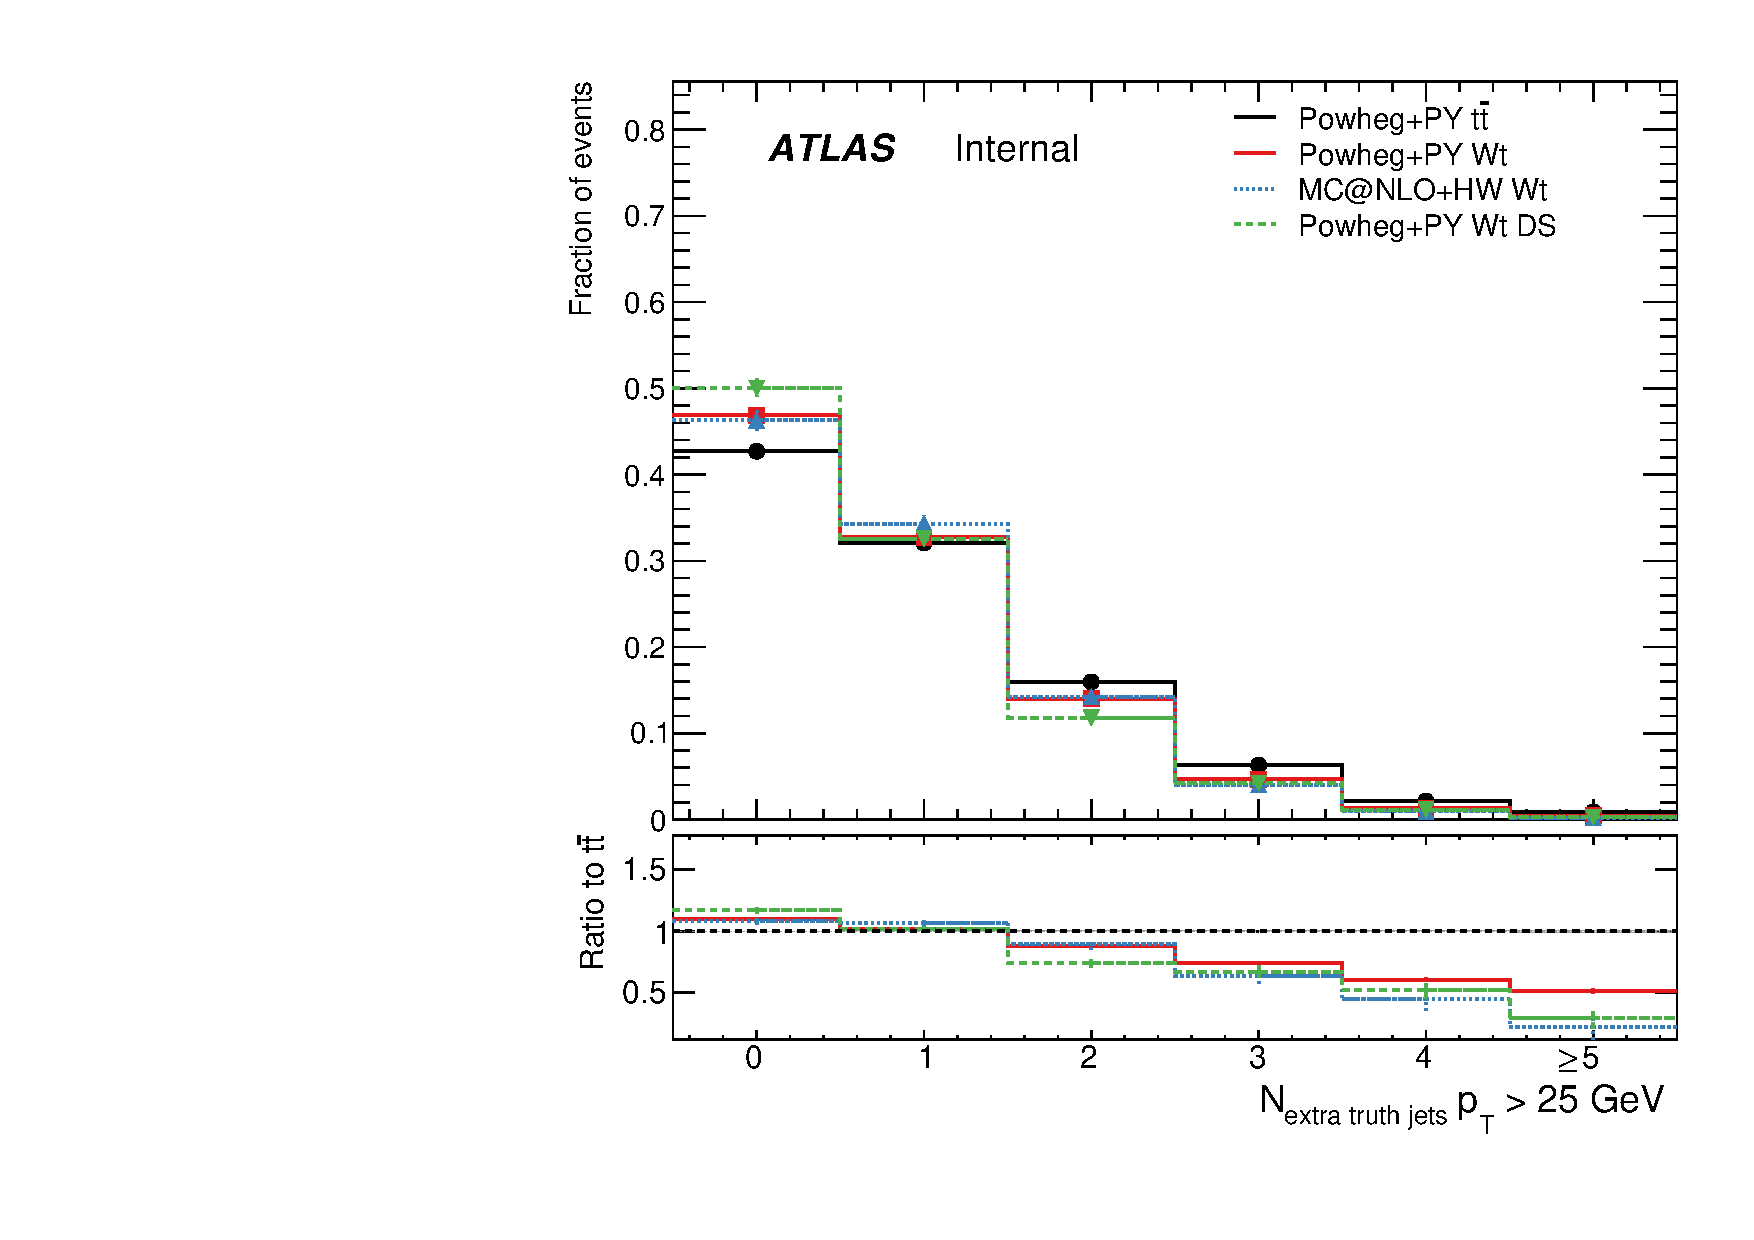
\includegraphics[width=\textwidth]{fig/MCComp/WtNTruthExtraJets25.pdf}
% \end{subfigure}
% \begin{subfigure}[]{0.45\textwidth}
% 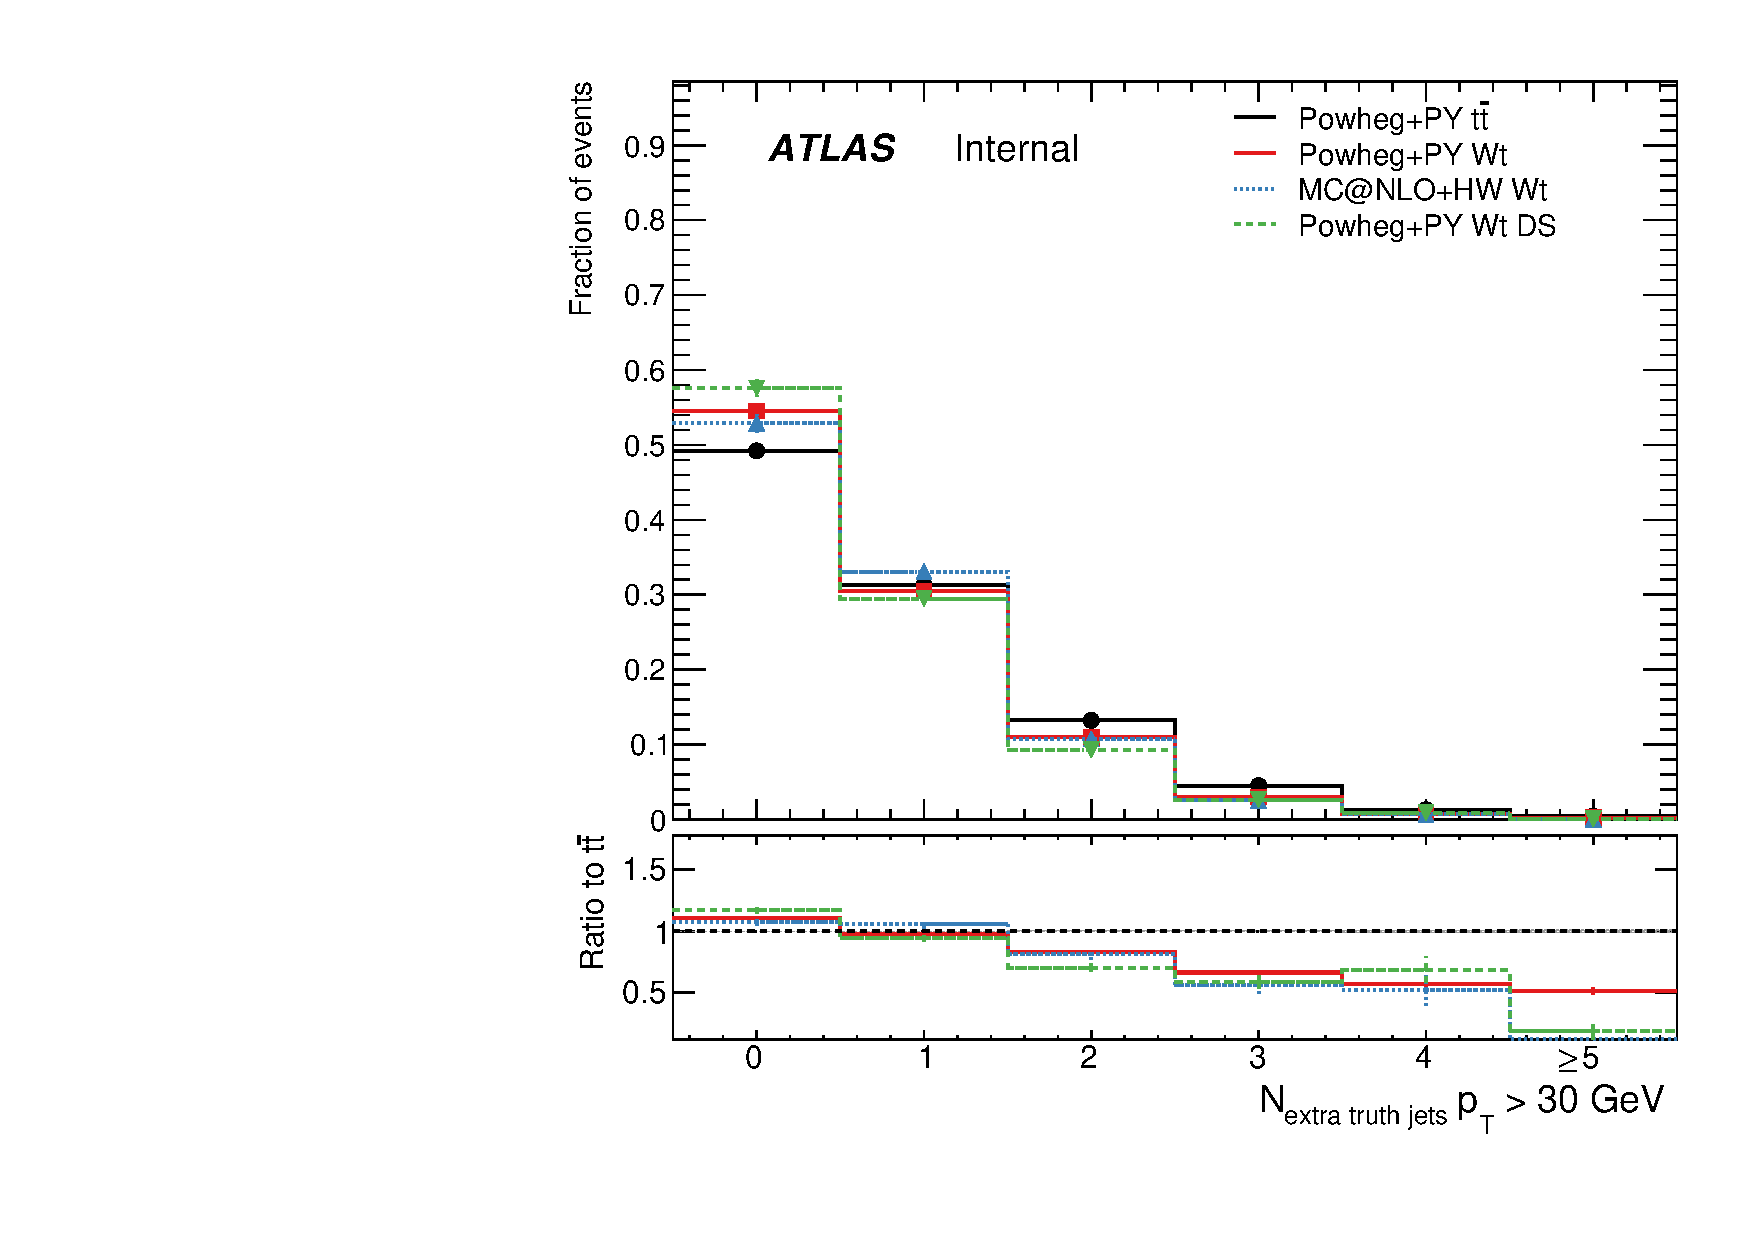
\includegraphics[width=\textwidth]{fig/MCComp/WtNTruthExtraJets30.pdf}
% \end{subfigure}
% \\
% \begin{subfigure}[]{0.45\textwidth}
% 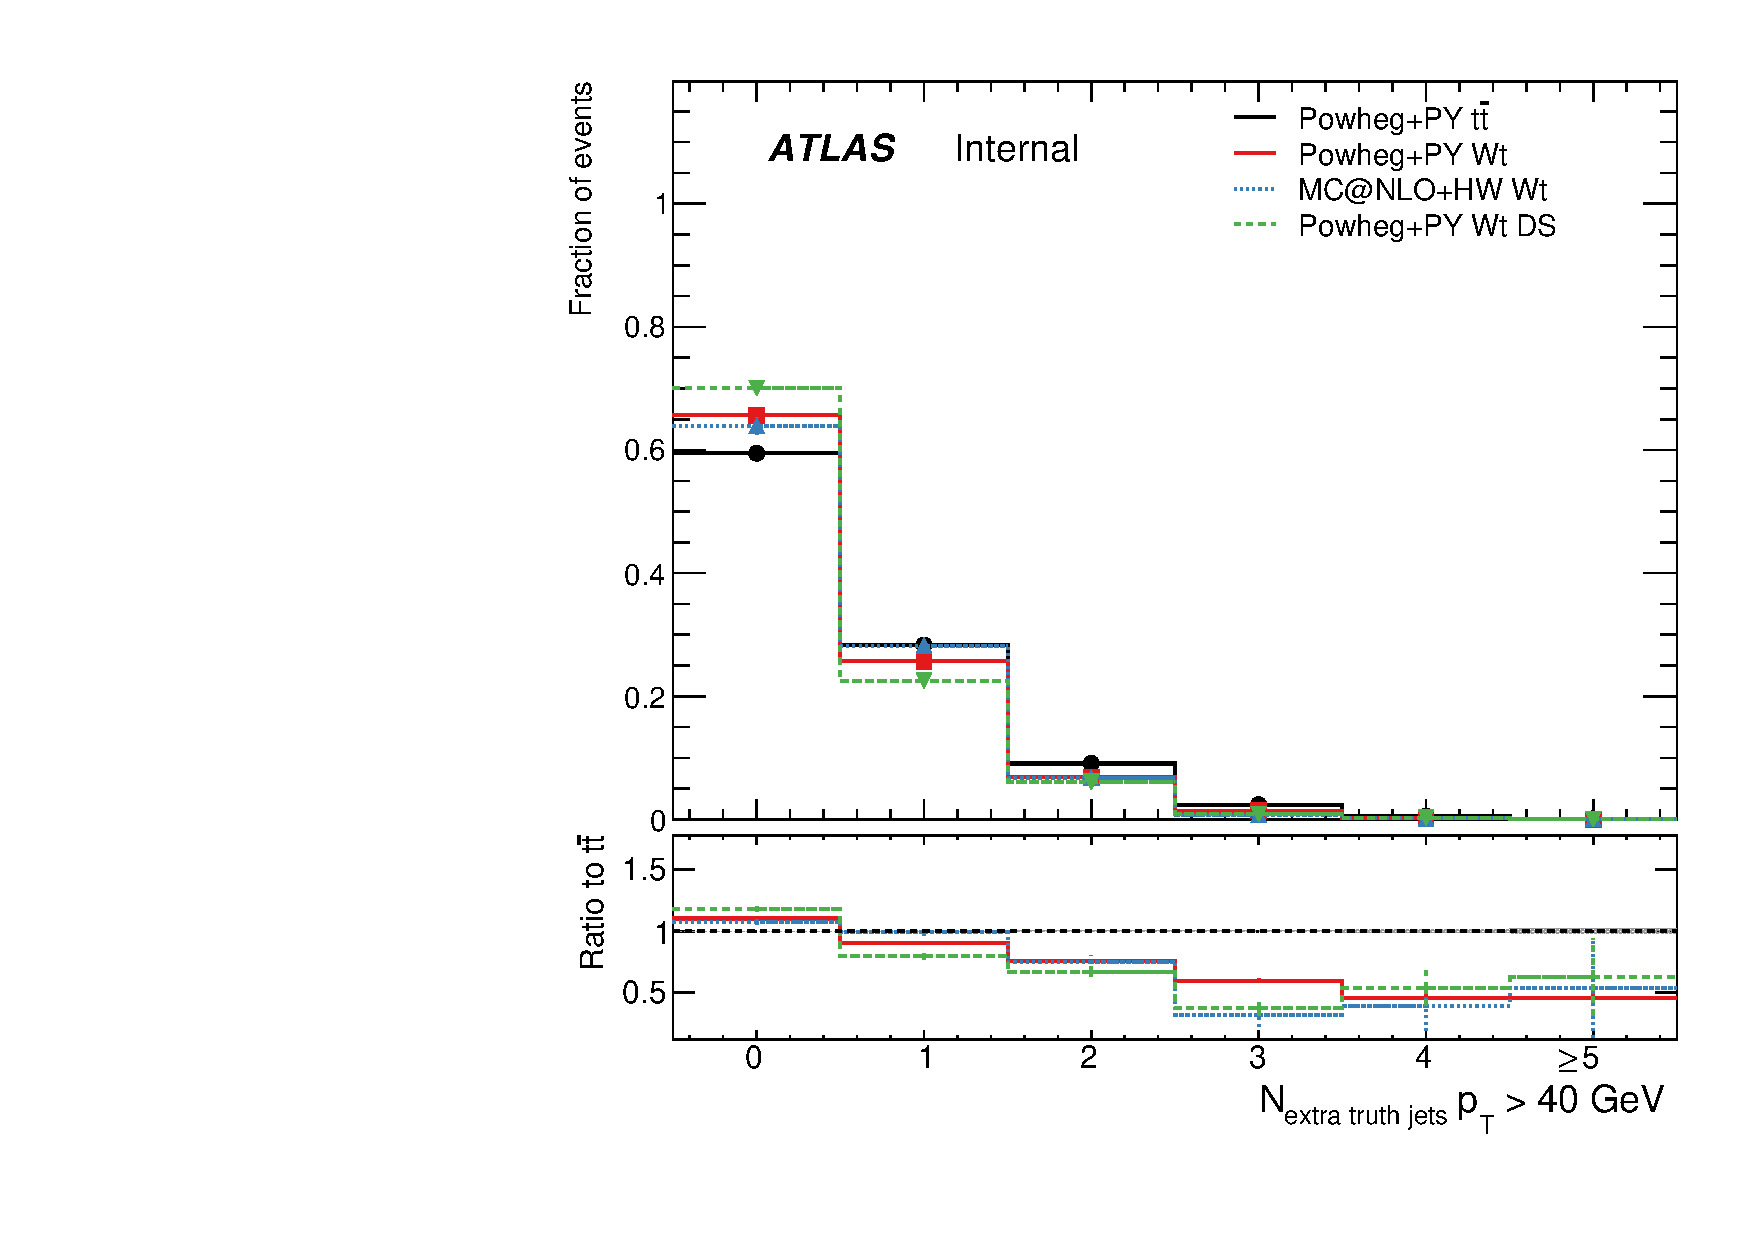
\includegraphics[width=\textwidth]{fig/MCComp/WtNTruthExtraJets40.pdf}
% \end{subfigure}
% \begin{subfigure}[]{0.45\textwidth}
% 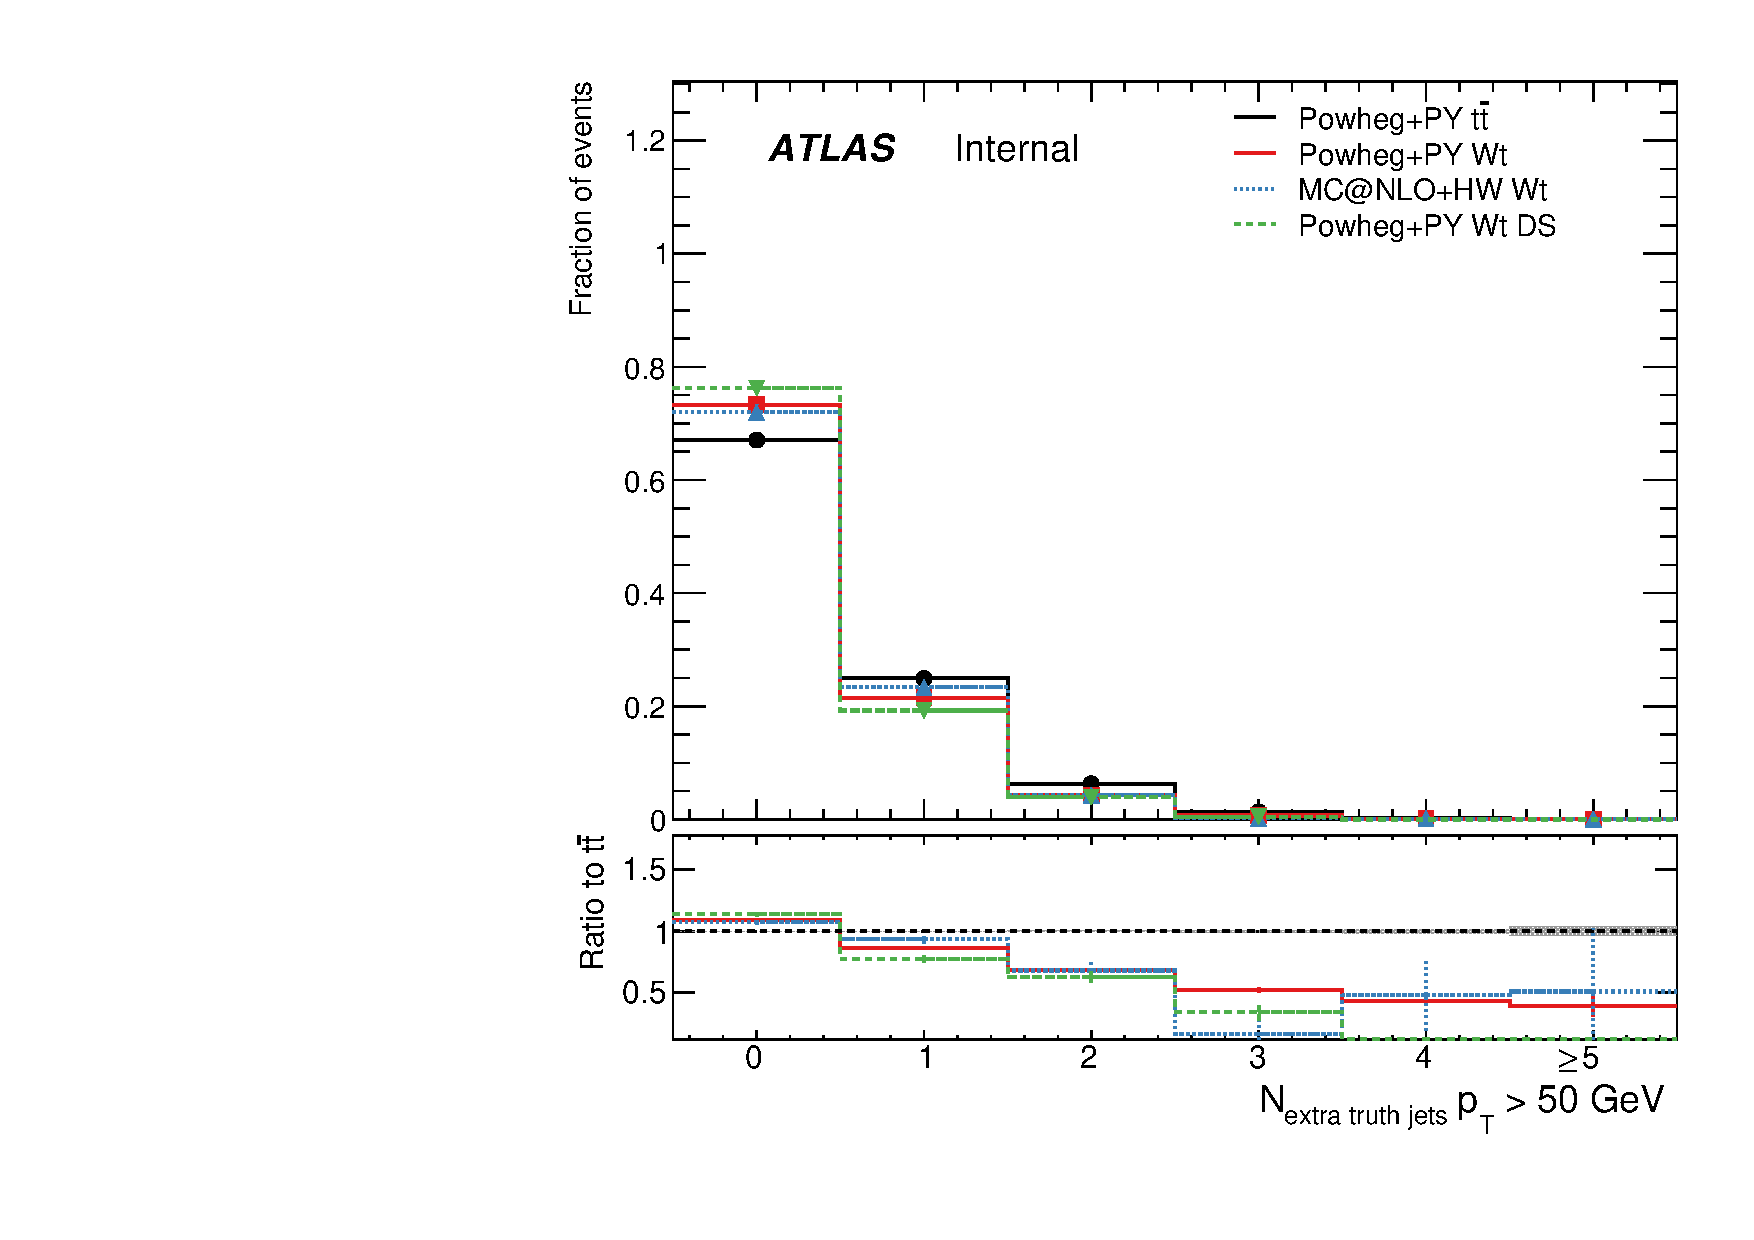
\includegraphics[width=\textwidth]{fig/MCComp/WtNTruthExtraJets50.pdf}
% \end{subfigure}
% \caption{Distributions of the number of extra truth jets with \pt > (a) 25, (b) 30, (c) 40 and (d) 50 \GeV in $Wt$ simulation. The distributions from various $Wt$ physics models are compared to \ttbar baseline simulation, each normalized by the number of selected truth events.}
% \label{fig:wtntruthjets}
% \end{figure}
% \begin{figure}
% \centering
% \begin{subfigure}[]{0.33\textwidth}
% 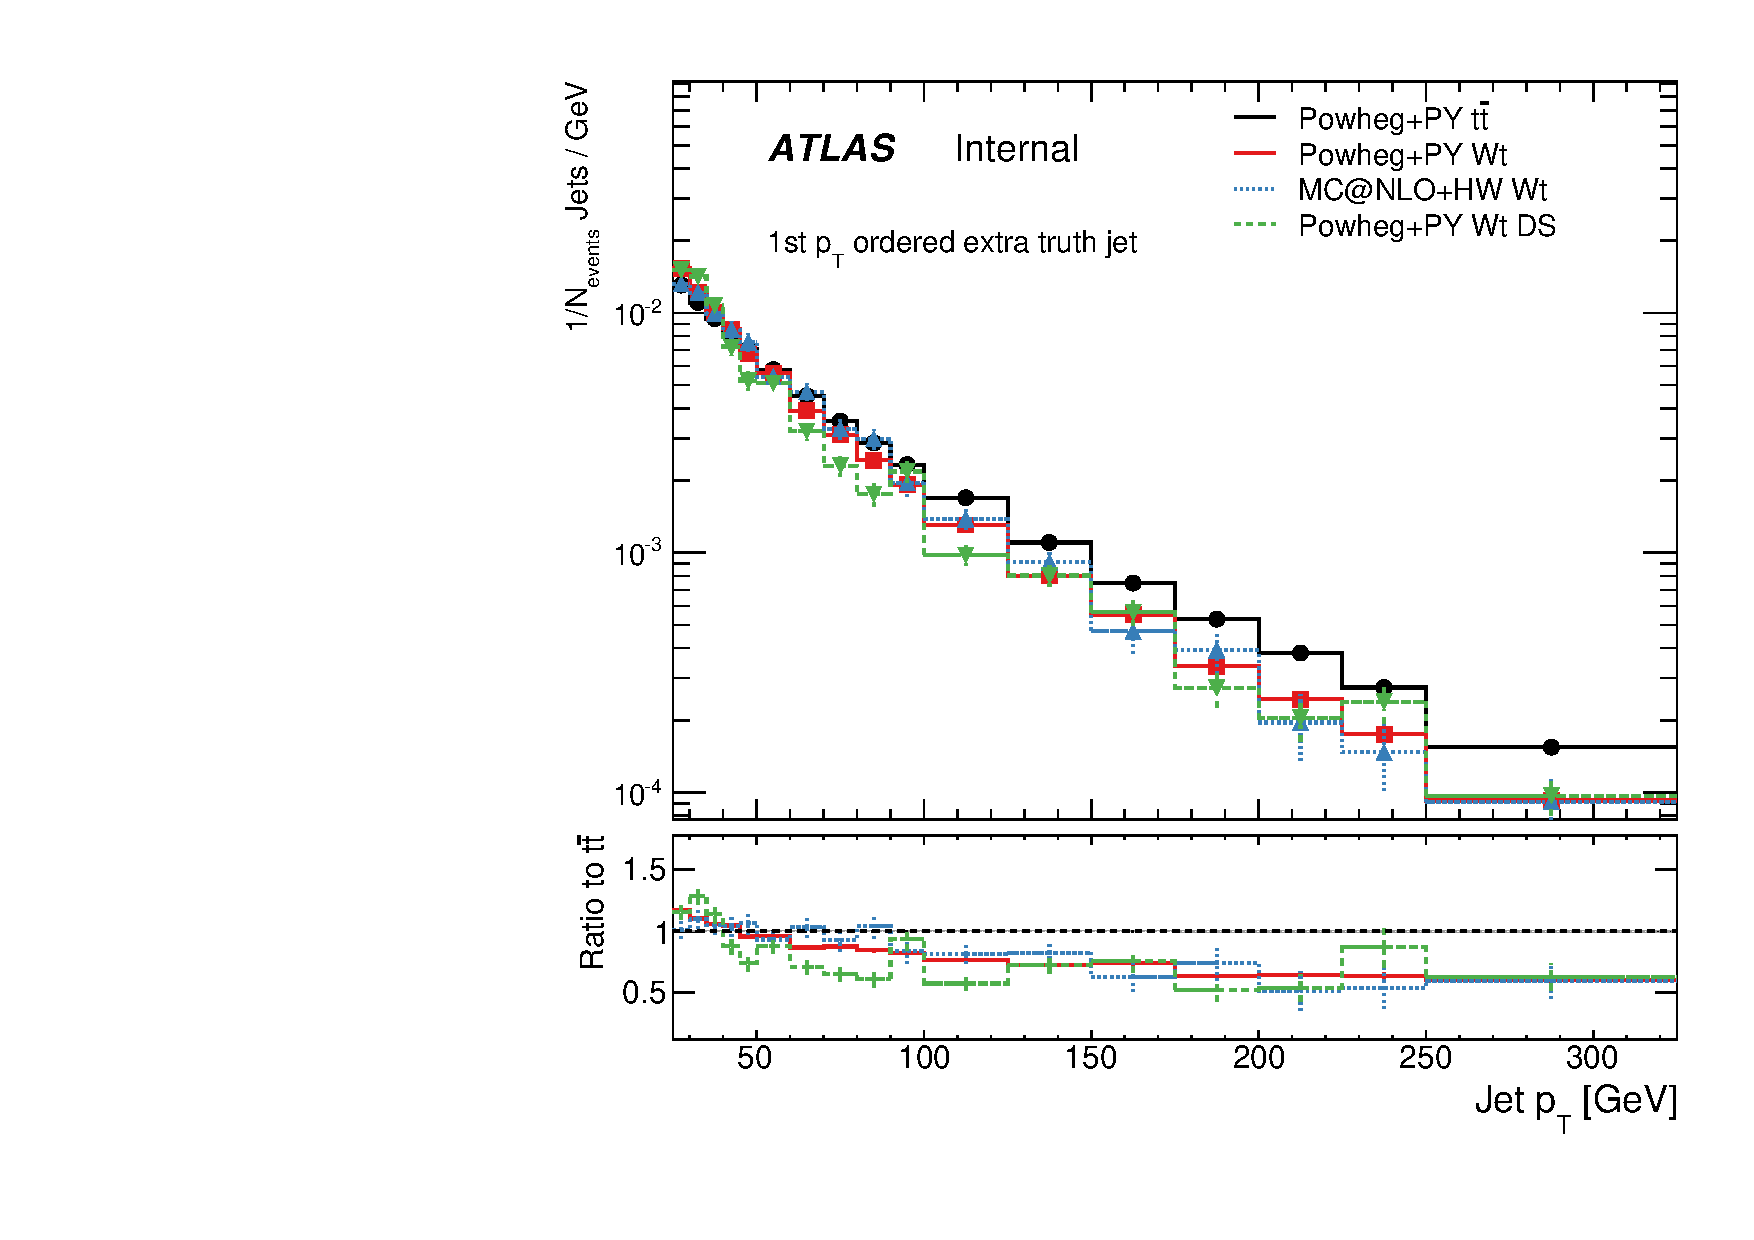
\includegraphics[width=\textwidth]{fig/MCComp/WtTruthPtJet0.pdf}
% \end{subfigure}
% \begin{subfigure}[]{0.33\textwidth}
% 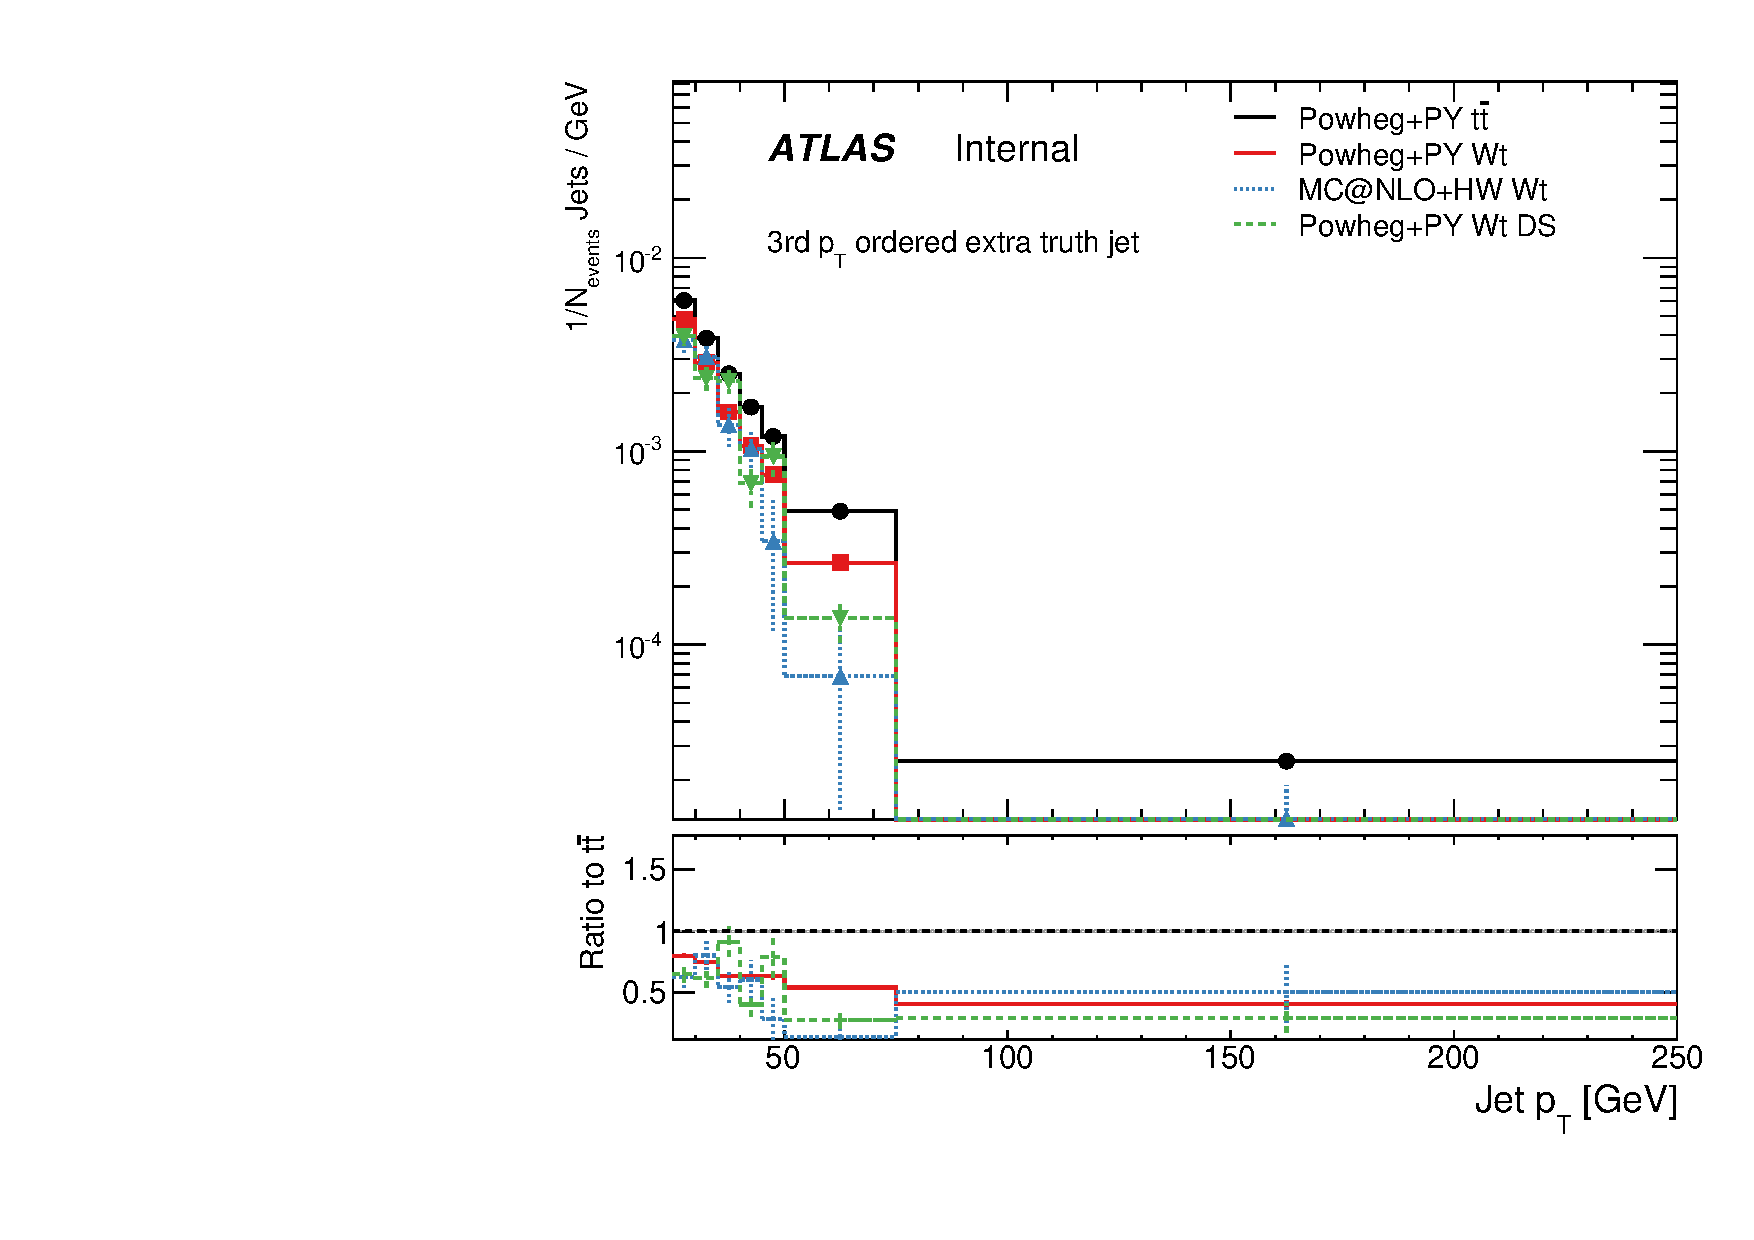
\includegraphics[width=\textwidth]{fig/MCComp/WtTruthPtJet2.pdf}
% \end{subfigure}
% \\
% \begin{subfigure}[]{0.33\textwidth}
% 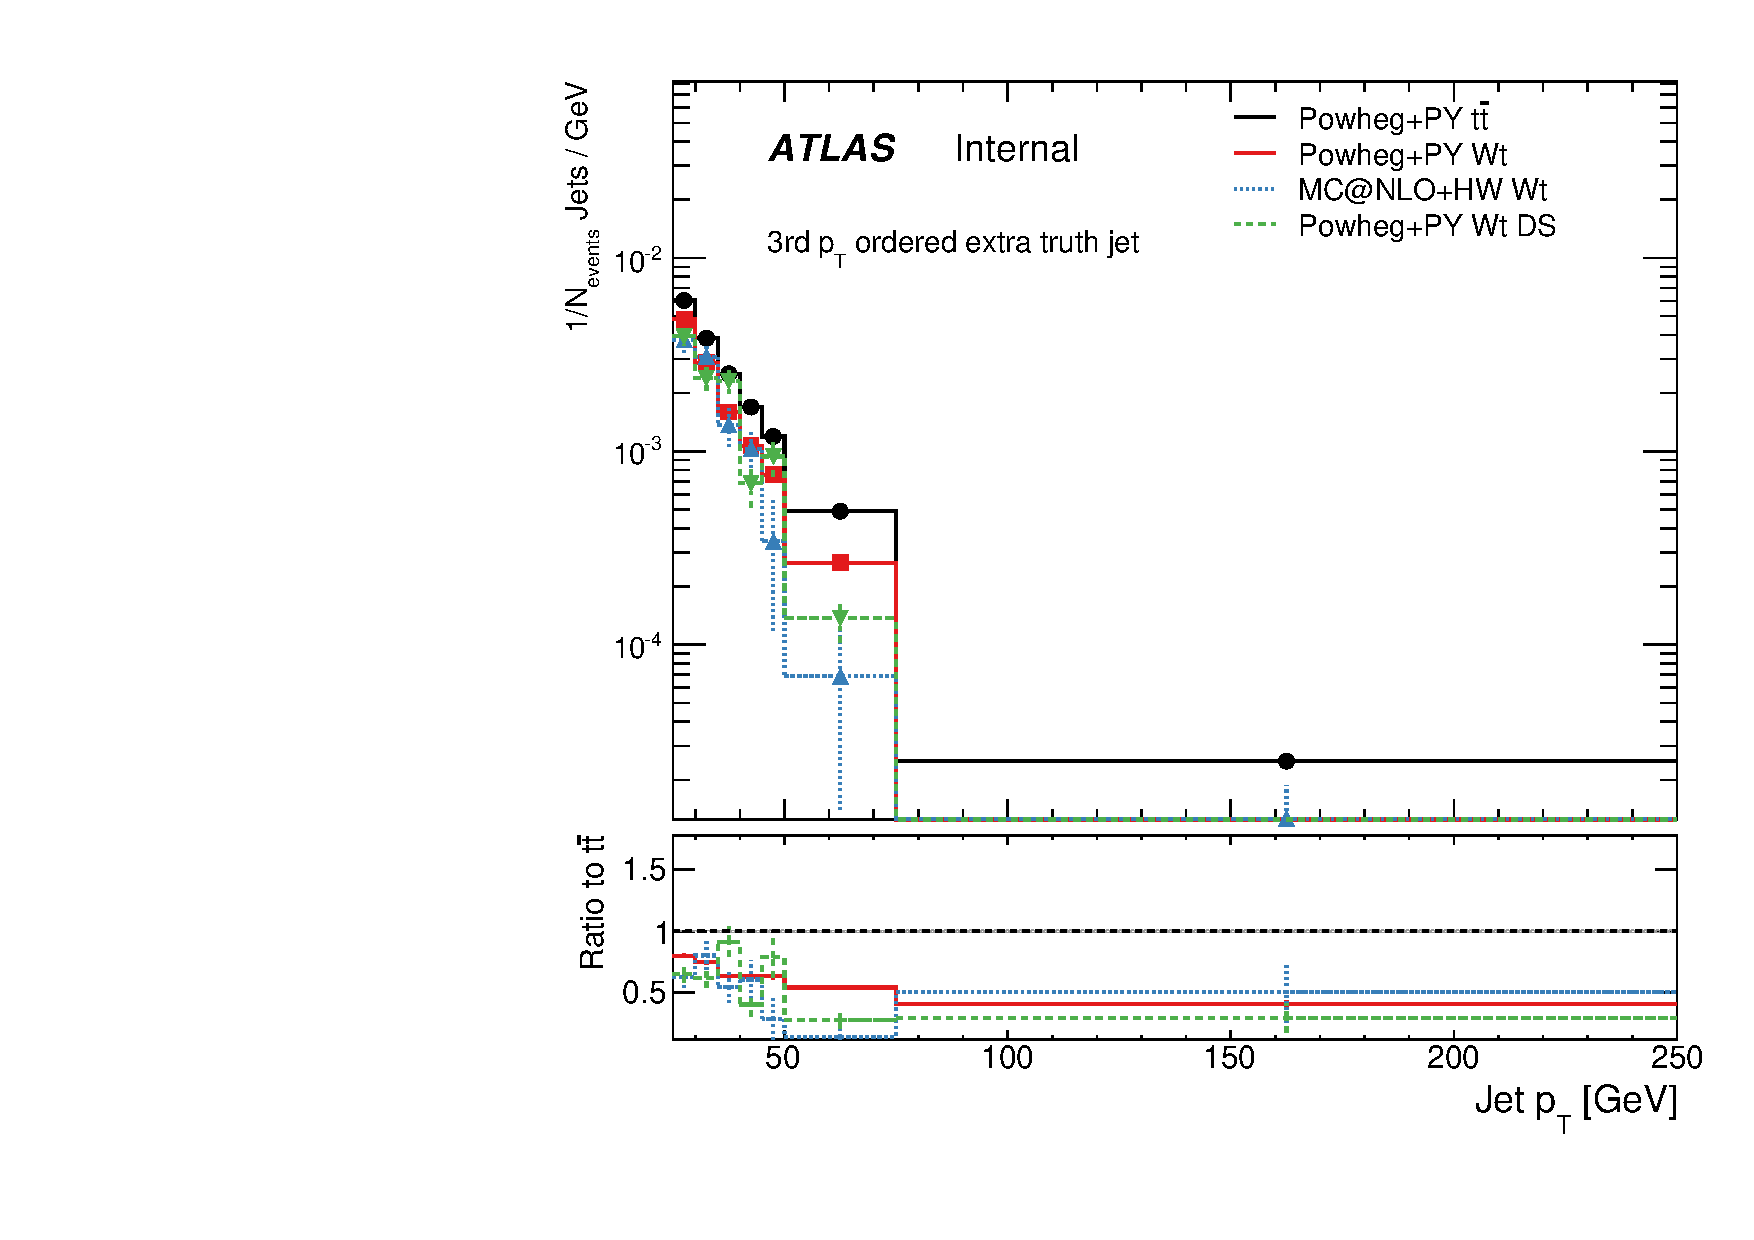
\includegraphics[width=\textwidth]{fig/MCComp/WtTruthPtJet2.pdf}
% \end{subfigure}
% \begin{subfigure}[]{0.33\textwidth}
% 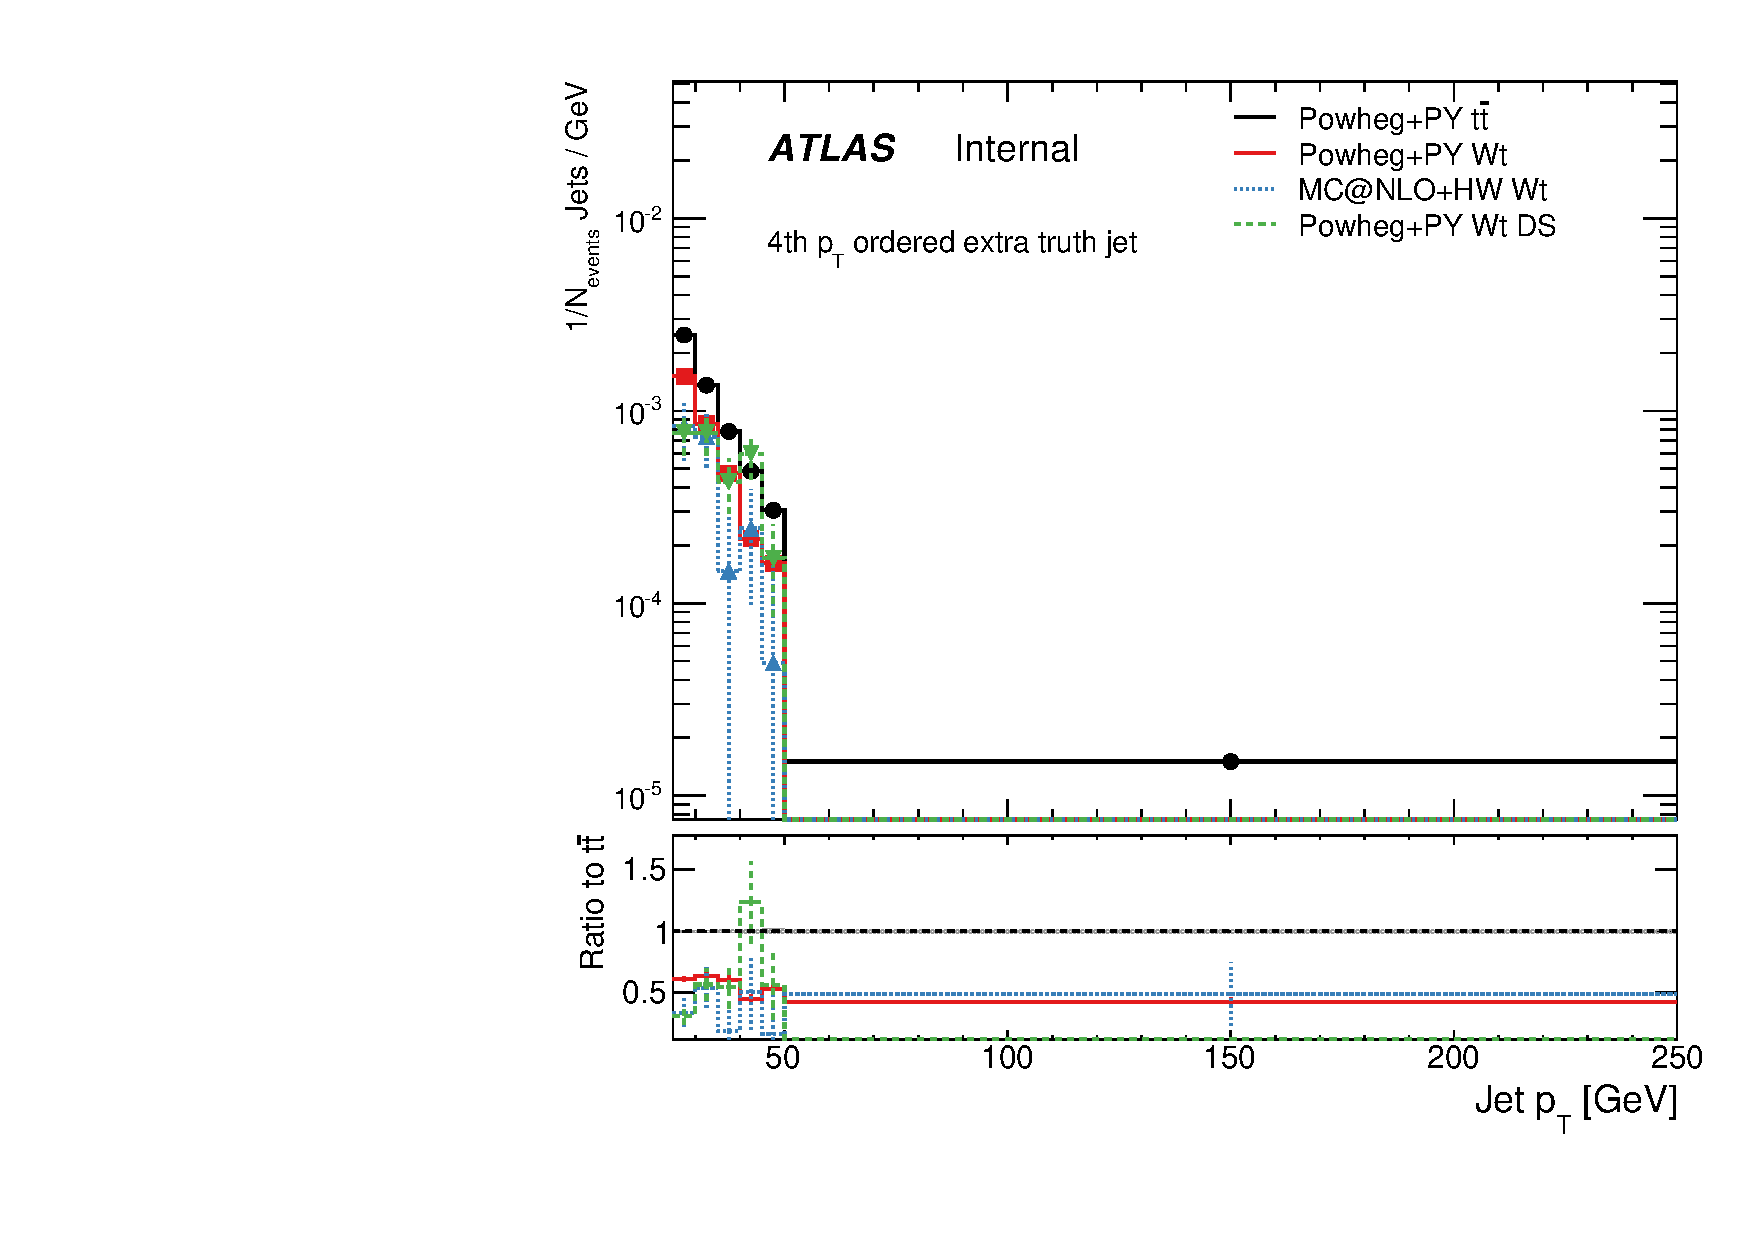
\includegraphics[width=\textwidth]{fig/MCComp/WtTruthPtJet3.pdf}
% \end{subfigure}
% \begin{subfigure}[]{0.33\textwidth}
% 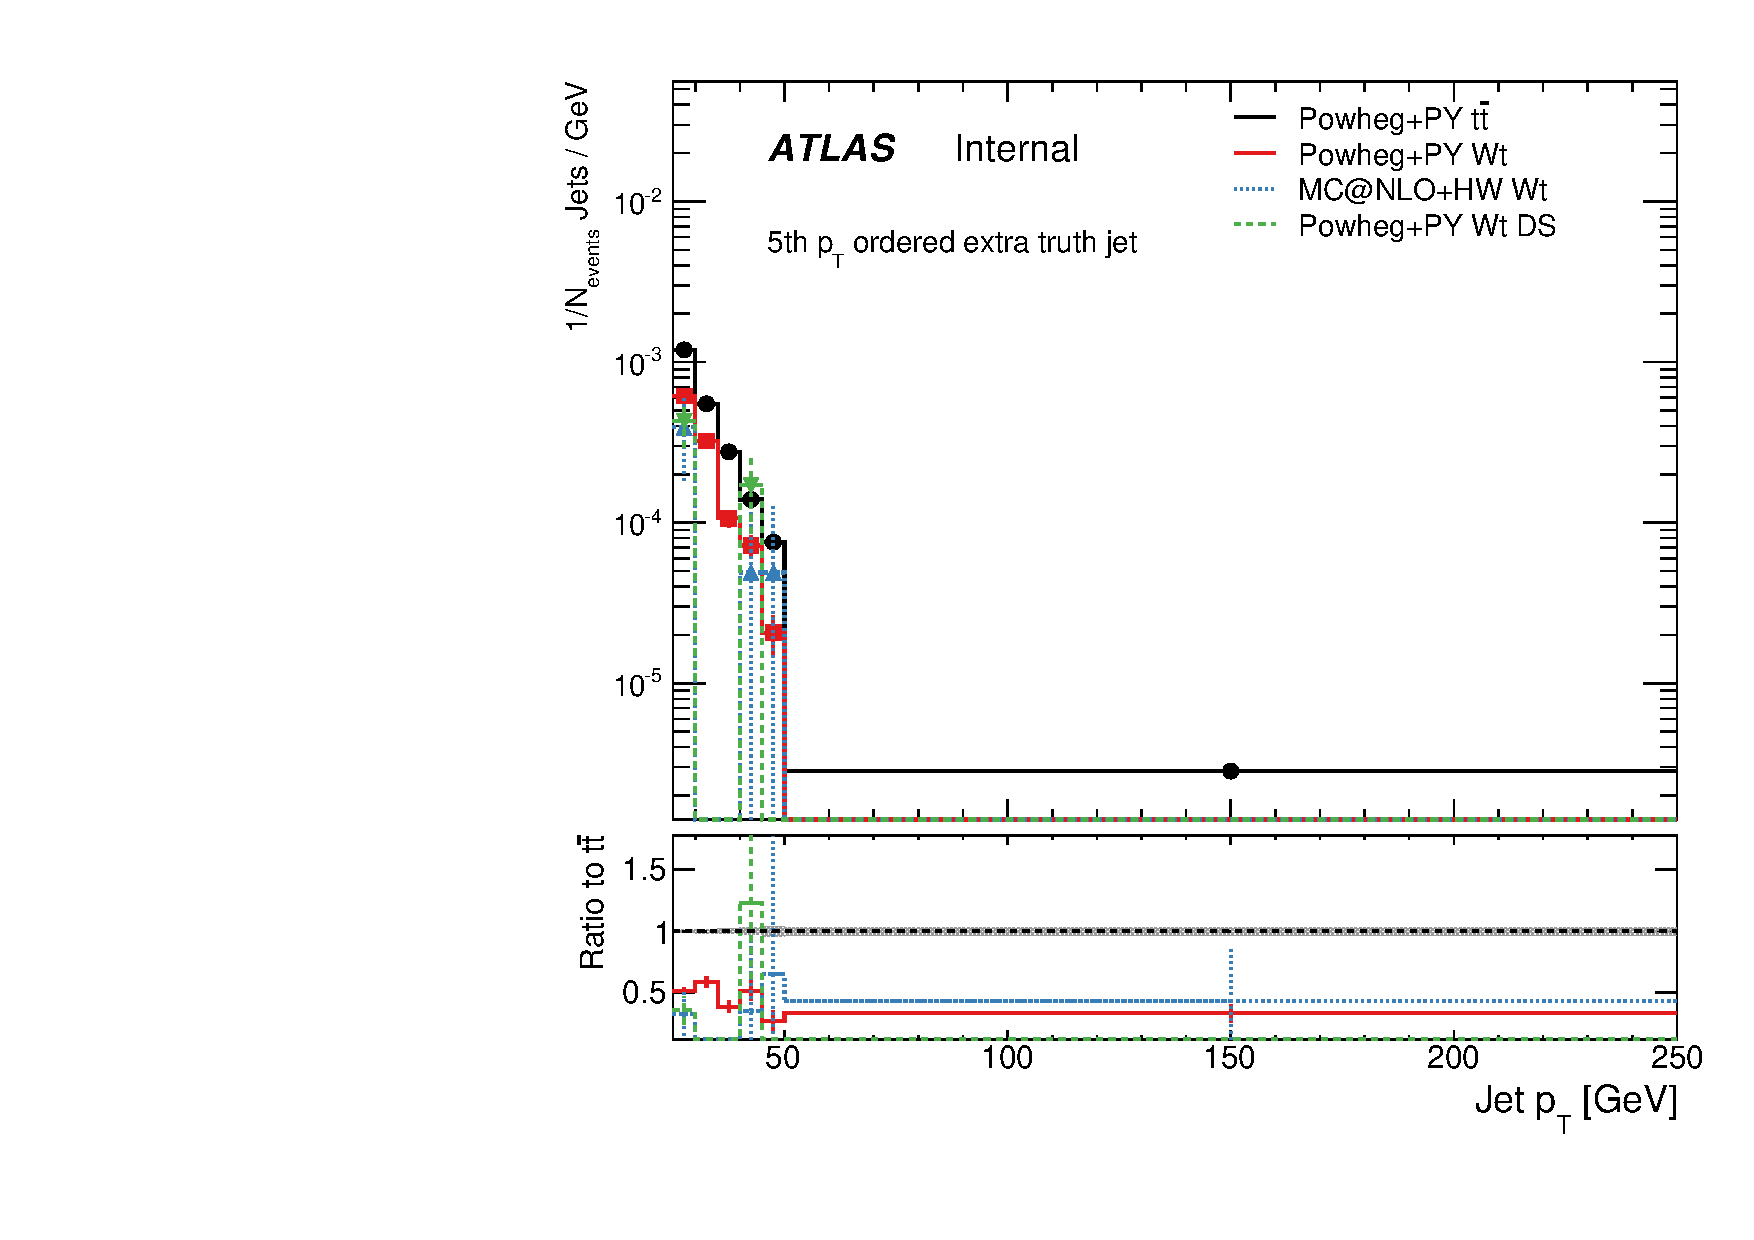
\includegraphics[width=\textwidth]{fig/MCComp/WtTruthPtJet4.pdf}
% \end{subfigure}
% \caption{Distributions of the extra truth jet \pt in $Wt$ simulation for jet ranks 1-5 (a-e). The distributions from $Wt$ are compared to \ttbar baseline simulation, each normalized by the number of selected truth events.}
% \label{fig:wttruthjetpt}
% \end{figure}

\clearpage
